\documentclass{article}
\usepackage{xcolor}
\usepackage{amsmath}
\usepackage{amsfonts}
\usepackage{tikz}
\begin{document}
\textbf{1351. (\color{red}d1\color{black}, 2022, Giochi di Archimede)} On the shore of a circular lake are three docks. On a map, they look like points $A, B, C$ on a circle and their angles can be measured to be $\angle CAB = 57^\circ$, $\angle ABC = 48^\circ$, $\angle BCA = 75^\circ$. In case a boat on the lake needs emergency, the nearest dock sends a rescue boat. What portion of the lake is assisted by the dock that covers the biggest area?

\textbf{1289. (\color{red}d1\color{black}, 2019 AIME I, P3 of 15)} In $\triangle PQR$, $PR=15$, $QR=20$, and $PQ=25$. Points $A$ and $B$ lie on $\overline{PQ}$, points $C$ and $D$ lie on $\overline{QR}$, and points $E$ and $F$ lie on $\overline{PR}$, with $PA=QB=QC=RD=RE=PF=5$. Find the area of hexagon $ABCDEF$.

\textbf{1281. (\color{red}d1\color{black}, 2022 NZMO1, P1 of 8)} \(ABCD\) is a rectangle with side lengths \(AB = CD = 1\) and \(BC = DA = 2\). Let \(M\) be the midpoint of \(AD\). Point \(P\) lies on the opposite side of line \(MB\) to \(A\), such that triangle \(MBP\) is equilateral. Find the value of \(\angle PCB\).

\textbf{1239. (\color{red}d1\color{black}, Alternate Segment Theorem)} Let \(ABC\) be a triangle with circumcircle \(\Gamma\).  Let \(\ell\) be a line tangent to \(\Gamma\) at \(B\), and let \(D\) be a point on \(\ell\) such that \(D\) and \(A\) are on opposite sides of \(BC\).  Prove that \(\angle BAC = \angle DBC\).

\textbf{1198. (\color{red}d1\color{black}, 2021 Irish MO, P2 of 10)} An isosceles triangle $ABC$ is inscribed in a circle with $\angle ACB = 90^o$ and $EF$ is a chord of the circle such that neither E nor $F$ coincide with $C$. Lines $CE$ and $CF$ meet $AB$ at $D$ and $G$ respectively. Prove that $|CE|\cdot |DG| = |EF| \cdot  |CG|$.

\textbf{1177. (\color{red}d1\color{black}, 2018 UK JMO, B4)} A rectangular sheet of paper is labelled $ABCD$, with $AB$ one of the longer sides. The sheet is folded so that vertex $A$ is placed exactly on top of the opposite vertex $C$. The fold line is $XY$, where $X$ lies on $AB$ and $Y$ lies on $CD$. Prove that triangle $CXY$ is isosceles.

\textbf{1127. (\color{red}d1\color{black}, 2016 Senior Maths Challenge, P24 of 25)} Let $PQRS$ be a square and let $U$ be the midpoint of $QR$.  The point $T$ lies on $SR$ such that the line $TU$ is tangent to the circle centred at $P$ with radius $PQ$. What is the ratio of the length of $TR$ to the length of $UR$?

\textbf{1043. (\color{red}d1\color{black}, 2018 AMC10, P15 of 25)} Two circles of radius 5 are externally tangent to eachother, and internally tangent to a circle of radius 13 at points $A$ and $B$, respectively. The distance $AB$ can be written as $\frac{m}{n}$, where $m$ and $n$ are relatively prime positive integers. What is $m + n$?

\textbf{1022. (\color{red}d1\color{black}, 1997 AMC12, P9 of 30)} Let $ABCD$ be a square of side length 2. If $E$ is the midpoint of $AD$, and $F$ is the foot of the perpendicular from $C$ to $BE$, what is the area of the quadrilateral $CDEF$?

\textbf{1008. (\color{red}d1\color{black}, 2018 AMC10B, P7 of 25)} $N$ congruent semicircles lie on the diameter of a large semicircle, with their diameters covering the diameter of the large semicircle with no overlap. Let $A$ be the combined area of the small semicircles, and $B$ the area inside the large semicircle but outside the small semicircles. If $A:B = 1:18$, what is $N$?

\textbf{959. (\color{red}d1\color{black}, 2004 SMC, P22 of 25, adapted)} Let $ABCD$ be a quadrilateral, with $AB$ parallel to $CD$ and lengths $\overline{AB}=x$ and $\overline{CD}=y$. Suppose $AC$ and $BD$ meet at $Z$. Suppose the line through $Z$ parallel to $AB$ meets $BC$ and $DA$ at $P$ and $Q$ respectively. Show that the length $\overline{PQ}$ can be determined just from the values of $x$ and $y$. Then find a formula for $\overline{PQ}$ in terms of $x$ and $y$.

\textbf{952. (\color{red}d1\color{black}, 2013 Bosnia \& Herzegovina Regional Grade 9, P2 of 4)} In a triangle $ABC$, $\angle ACB = 50^\circ$ and $\angle CBA = 70^\circ$. Let $D$ be the foot of the perpendicular from point $A$ to side $BC$ and $E$ the antipode of $A$ in the circumcircle of $ABC$. Find $\angle DAE$.

\textbf{854. (\color{red}d1\color{black}, 2019 ASC, P1 of 5)} For $n \geq 3$, the sequence of points $A_{1}, A_{2}, \ldots, A_{n}$ in the Cartesian plane has increasing $x$ -coordinates. The line $A_{1} A_{2}$ has positive gradient, the line $A_{2} A_{3}$ has negative gradient, and the gradients continue to alternate in sign, up to the line $A_{n-1} A_{n} .$ So the zigzag path $A_{1} A_{2} \cdots A_{n}$ forms a sequence of alternating peaks and valleys at $A_{2}, A_{3}, \ldots, A_{n-1}$
\smallbreak
The angle less than $180^{\circ}$ defined by the two line segments that meet at a peak is called a peak angle. Similarly, the angle less than $180^{\circ}$ defined by the two line segments that meet at a valley is called a valley angle. Let $P$ be the sum of all the peak angles and let $V$ be the sum of all the valley angles.
\smallbreak
Prove that if $P \leq V$, then $n$ must be even.

\textbf{784. (\color{red}d1\color{black}, Folklore)} Let $M$ be the midpoint of side $BC$ of triangle $ABC.$ Prove that $AB + AC > 2AM.$

\textbf{764. (\color{red}d1\color{black}, 2018 UK IMOK, M6)} Let $ABC$ be a triangle. Let points $T$ and $U$ lie on segment $AB$, $P$ and $Q$ lie on segment $BC$ and $R$ and $S$ lie on segment $CA$. Suppose $SP$ and $AB$ are parallel, $UR$ and $BC$ are parallel, and $QT$ and $CA$ are parallel. Suppose also that $SP$, $UR$ and $QT$ also meet at a point. Suppose also that the lengths $PQ$, $RS$ and $TU$ are equal. Prove that $$\frac{1}{PQ} = \frac{1}{AB} + \frac{1}{BC} + \frac{1}{CA}.$$

\textbf{763. (\color{red}d1\color{black}, 2015 BMO1, P2 of 6)} Let $ABCD$ be a cyclic quadrilateral and let the lines $CD$ and $BA$ meet at $E$. The line through $D$ which is tangent to the circle $ADE$ meets the line $CB$ at $F$. Prove that the triangle $CDF$ is isosceles.

\textbf{735. (\color{red}d1\color{black}, 2015 UK JMO, B4)} The point $F$ lies inside the regular pentagon $ABCDE$ so that $ABFE$ is a rhombus. Prove that $EFC$ is a straight line.

\textbf{700. (\color{red}d1\color{black}, Thales' theorem and converse)} Points \(A\), \(B\), and \(C\) lie on a circle \(\Gamma\). Show that \(\angle ABC = 90^\circ\) if and only if \(AC\) is the diameter of \(\Gamma\).

\textbf{581. (\color{red}d1\color{black}, 2016 UK IMOK, C4)} The diagram shows an equilateral triangle $A B C$ and two squares $A W X B$ and $A Y Z C$.
Prove that triangle $A X Z$ is equilateral.

\begin{center}
    \tikzset{every picture/.style={line width=0.75pt}} %set default line width to 0.75pt        

    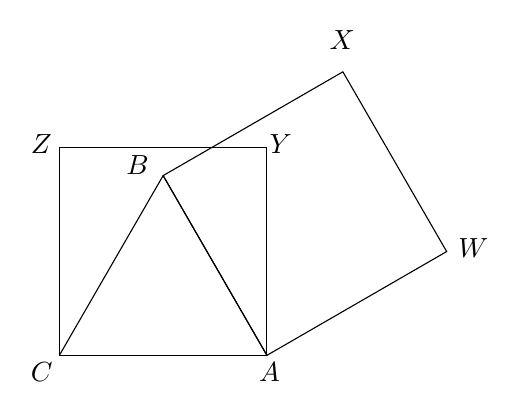
\begin{tikzpicture}[x=0.75pt,y=0.75pt,yscale=-1,xscale=1]
        %uncomment if require: \path (0,300); %set diagram left start at 0, and has height of 300

        %Shape: Square [id:dp7912356786882051] 
        \draw   (96,110) -- (196,110) -- (196,210) -- (96,210) -- cycle ;
        %Shape: Boxed Line [id:dp7833385391080145] 
        \draw    (146,123.4) -- (96,210) ;
        %Shape: Boxed Line [id:dp7553088933468859] 
        \draw    (146,123.4) -- (196,210) ;
        %Shape: Square [id:dp5436818718555383] 
        \draw   (232.6,73.4) -- (282.6,160) -- (196,210) -- (146,123.4) -- cycle ;

        % Text Node
        \draw (81,212.4) node [anchor=north west][inner sep=0.75pt]    {$C$};
        % Text Node
        \draw (191,212.4) node [anchor=north west][inner sep=0.75pt]    {$A$};
        % Text Node
        \draw (127,112.4) node [anchor=north west][inner sep=0.75pt]    {$B$};
        % Text Node
        \draw (81,102.4) node [anchor=north west][inner sep=0.75pt]    {$Z$};
        % Text Node
        \draw (196,102.4) node [anchor=north west][inner sep=0.75pt]    {$Y$};
        % Text Node
        \draw (287,152.4) node [anchor=north west][inner sep=0.75pt]    {$W$};
        % Text Node
        \draw (225,52.4) node [anchor=north west][inner sep=0.75pt]    {$X$};
    \end{tikzpicture}
\end{center}

\textbf{497. (\color{red}d1\color{black}, 2020 NZMO1, P2 of 8)} Let $ABCD$ be a square and let $ X $ be any point on side $ BC $ between $ B $ and $ C $ .  Let $ Y $ be the point on line $ CD $ such that $ BX=YD $ and $ D $ is between $ C $ and $ Y $ .  Prove that the midpoint of $ XY $ lies on diagonal $ BD $ .

\textbf{1366. (\color{red}d2\color{black}, 1989 Cono Sur Olympiad, P1 of 6)} Two isosceles triangles with sidelengths $x,x,a$ and $x,x,b$ ($a \neq b$) have equal areas. Find $x$.

\textbf{1352. (\color{red}d2\color{black}, Power of a Point)} Let $\Gamma$ be a circle and $P$ be a point not on the circumference of $\Gamma$. Suppose that a line $\ell$ through $P$ either intersects $\Gamma$ at two distinct points $A$ and $B$, or it is tangent to $\Gamma$, making $A$ and $B$ the same point. Prove that $PA \times PB$ is independent of $\ell$.

\textbf{1344. (\color{red}d2\color{black}, 1997 CMO, P4 of 5)} Let $ABCD$ be a parallelogram, and $P$ a point in its interior. Show that, if $\angle APB + \angle CPD = 180^\circ$, then $\angle PBC = \angle PDC$.

\textbf{1310. (\color{red}d2\color{black}, 2021 IOQM)} A bug travels in the coordinate plane moving only along the lines that are parallel to the $x$-axis or $y$-axis. Let $A=(-3,2)$ and $B=(3,-2)$. Consider all possible paths of the bug from $A$ to $B$ of length at most $14$. How many points with integer coordinates lie on at least one of these paths?

\textbf{1303. (\color{red}d2\color{black}, 2013 HMMT)} Let triangle $ABC$ satisfy $2BC = AB + AC$ and have incenter $I$ and circumcircle $\omega$. Let $D$ be the intersection of $AI$ and $\omega$ (with $A, D$ distinct). Prove that $I$ is the midpoint of $AD$.

\textbf{1267. (\color{red}d2\color{black}, Folklore)} Let $ABC$ be a triangle, and $L$, $M$ and $N$ the midpoints of $BC$, $CA$ and $AB$, respectively. Prove that $\angle LAC = \angle ABM$ if, and only if, $\angle ANC = \angle ALB$.

\textbf{1205. (\color{red}d2\color{black}, PST 4.6)} In rectangle \(ABCD\), let \(M\) and \(N\) be the midpoints of \(BC\) and \(CD\), respectively.  Let \(DM\) and \(BN\) intersect at \(P\).

Prove that \(\angle MAN = \angle BPM\).

\textbf{1170. (\color{red}d2\color{black}, 2018 Austria Beginners' Competitions, P2 of 4)} Let $ABC$ be an acute-angled triangle, $M$ the midpoint of the side $AC$ and $F$ the foot on $AB$ of the altitude through the vertex $C$. Prove that $AM = AF$ holds if and only if $\angle BAC = 60^o$.

\textbf{1155. (\color{red}d2\color{black}, Pitot's theorem)} Prove that a quadrilateral with side lengths $a, b, c, d$, in that order, has an inscribed circle if, and only if, $a + c = b + d$.

\textbf{1106. (\color{red}d2\color{black}, 1997 BMO1, P4 of 5)} Let $ABCD$ be a convex quadrilateral. The midpoints of $AB$, $BC$, $CD$ and $DA$ are $P$, $Q$, $R$, and $S$, respectively. Given that the quadrilateral $PQRS$ has area 1, prove that the area of the quadrilateral $ABCD$ is 2.

\textbf{1085. (\color{red}d2\color{black}, Pi)} Let $C$ be a circle of diameter 1. Show that the length of the circumference of $C$ is bigger than 3, but smaller than 4.

\textbf{1078. (\color{red}d2\color{black}, 2003 BMO1, P2 of 5)} $ABCD$ is a rectangle, $P$ is the midpoint of $AB$, and $Q$ is the point on $PD$ such that $CQ$ is perpendicular to $PD$. Prove that the triangle $BQC$ is isosceles.

\textbf{1057. (\color{red}d2\color{black}, 2018 Polish Junior MO Round 2, P2 of 5)} Let $ABC$ be an acute angled triangle with $AC \ne BC$. Let $K$ be the foot of the altitude from $C$, and $O$ be the circumcentre of $ABC$. Show that the quadrilaterals $AKOC$ and $BKOC$ have the same area.

\textbf{988. (\color{red}d2\color{black}, 2021 ICMC Round 1, P1 of 6)} Let $T_{n}$ be the number of non-congruent triangles with positive area and integer side lengths summing to $n$. Prove that $T_{2022}=T_{2019}$.

\textbf{889. (\color{red}d2\color{black}, 2019 IGO Elementary, P4)} Quadrilateral $ABCD$ is given such that $$\angle DAC = \angle CAB = 60^\circ,$$ and
$$AB = BD - AC.$$ Lines $AB$ and $CD$ intersect each other at point $E$. Prove that \[
    \angle ADB = 2\angle BEC.\]

\textbf{868. (\color{red}d2\color{black}, 2021 NZMO1, P2)} Let \(ABCD\) be a trapezium such that \(AB \parallel CD\). Let \(E\) be the intersection of diagonals \(AC\) and \(BD\). Suppose that \(AB = BE\) and \(AC = DE\). Prove that the internal angle bisector of \(\angle BAC\) is perpendicular to \(AD\).

\textbf{841. (\color{red}d2\color{black}, 2000 BMO1, P3 of 5)} Triangle $ABC$ has a right angle at $A$. Among all points $P$ on the perimeter of the triangle, find the position of $P$ such that $$AP+BP+CP$$ is minimised.

\textbf{826. (\color{red}d2\color{black}, 2000 BMO1, P1 of 5)} Two intersecting circles $C_1$ and $C_2$ have a common tangent which touches $C_1$ at $P$ and $C_2$ at $Q$. The two circles intersect at $M$ and $N$, where $N$ is nearer to $PQ$ than $M$ is. The line $PN$ meets the circle $C_2$ again at $R$. Prove that $MQ$ bisects angle $PMR$.

\textbf{806. (\color{red}d2\color{black}, Centroid)} Let $ABC$ be a triangle, and let $D$, $E$ and $F$ be the midpoints of $BC$, $CA$ and $AB$ respectively. Prove that $AD$, $BE$ and $CF$ meet at a point. If this point is $G$, prove that $AG$ is twice the length of $GD$.

\textbf{785. (\color{red}d2\color{black}, Catriona Shearer's Twitter)} A point $P$ is chosen on the diagonal $BD$ of square $ABCD.$ If $DP = CP + BP$ then find all possibilities for the value of $\angle CPD.$

\textbf{729. (\color{red}d2\color{black}, Folklore)} Let $ABCD$ be a convex quadrilateral with perpendicular diagonals which intersect at $P$. Prove that the reflections of $P$ across $AB$, $BC$, $CD$ and $DA$ form the vertices of a cyclic quadrilateral.

\textbf{715. (\color{red}d2\color{black}, Folklore)} A Platonic solid is a three-dimensional convex shape where all faces are congruent regular polygons, and each vertex has the same number of faces adjacent to it. Prove that, if we count two similar Platonic solids as not distinct, there are at most five distinct Platonic solids.

\textbf{687. (\color{red}d2\color{black}, Folklore)} Let $ABC$ be a triangle. Let $O$ be the centre of the circle $S$ that goes through $A$, $B$ and $C$. Let $A'$ be diametrically opposite $A$ on $S$. Let $B'$ be diametrically opposite $B$ on $S$. Let $C'$ be diametrically opposite $C$ on $S$. Prove that there exists a point $H$ such that $BA'CH$, $CB'AH$ and $AC'BH$ are all parallelograms.

\textbf{658. (\color{red}d2\color{black}, Praslov Problem 2.88)} Let $ABC$ be a triangle with circumcenter $O$. The foot of the altitude from $A$ is $H$. Prove that $\angle OAH = |\angle B - \angle C|$.

\textbf{652. (\color{red}d2\color{black}, Folklore)} Let $ABC$ be a triangle with incircle $\omega$, tangent to $AB$ at $X$, $BC$ at $Y$ and $CA$ at $Z$. The line $XY$ intersects the circle at $A$ through $Z$ at point $P$ and the circle at $C$ through $Z$ at point $Q$. Prove that $\angle PZX = \angle YZQ$.



\textbf{630. (\color{red}d2\color{black}, 2020 BMO1, P5 of 7)} Let points $A, B$ and $C$ lie on a circle $\Gamma .$ Circle $\Delta$ is tangent to $A C$ at $A .$ It meets $\Gamma$ again at $D$ and the line $A B$ again at $P .$ The point $A$ lies between points $B$ and $P .$ Prove that if $A D=D P,$ then $B P=A C .$

\textbf{617. (\color{red}d2\color{black}, 2013/4 BMO1, P2 of 6)} In the acute-angled triangle $ABC$, the foot of the perpendicular from $B$ to $CA$ is $E$. Let $\ell$ be the tangent to the circle $ABC$ at $B$. The foot of the perpendicular from $C$ to $\ell$ is $F$. Prove that $EF$ is parallel to $AB$.

\textbf{616. (\color{red}d2\color{black}, Varignon's Theorem)} Prove that the midpoints of the sides of a quadrilateral are the vertices of a parallelogram.

\textbf{504. (\color{red}d2\color{black}, Simson Line)} Let $A B C$ be a triangle and $P$ be any point on the circumcircle of $ABC$. Let $X$, $Y$, $Z$ be the feet of the perpendiculars from $P$ onto lines $B C$, $C A$, and $A B$. Prove that points $X, Y, Z$ are collinear.

\textbf{371. (\color{red}d2\color{black}, 2020 Maynooth Olympiad, P8 of 10 )} Two circles touch at a point \(T\) and have a common tangent \(P S\) If \(P Q\) is the diameter of circle 1 and \(Q R\) is tangent to circle \(2,\) show that \(P Q=Q R\).

\textbf{351. (\color{red}d2\color{black}, 2020 AMO, Q6 of 8)} Let $ABCD$ be a square. For a point $P$ inside $ABCD$, a \textit{windmill} centered at $P$ consists of two perpendicular lines $\ell_1$ and $\ell_2$ passing through P, such that
\begin{enumerate}
    \item $\ell_1$ intersects the sides $AB$ and $CD$ at $W$ and $Y$ respectively, and
    \item $\ell_2$ intersects the sides $BC$ and $DA$ at $X$ and $Z$ respectively. \end{enumerate}
A windmill is called \textit{round} if the quadrilateral $WXYZ$ is cyclic. \\
Determine all points $P$ inside $ABCD$ such that every windmill centered at $P$ is round.

\textbf{273. (\color{red}d2\color{black}, LuMaT 2018 Pre-eliminary Round)} Given a convex cyclic hexagon with side length of $1,1,1,1,2,2$ (in that particular order). Find all possible values of the radius of circumcircle from that hexagon.

\textbf{231. (\color{red}d2\color{black}, 2019 Oral Moscow Geometry Olympiad, Grade 8--9)} In the triangle $ABC, I$ is the center of the inscribed circle, point $M$ lies on the side of $BC$, with $\angle BIM = 90^o$. Prove that the distance from point $M$ to line $AB$ is equal to the diameter of the circle inscribed in triangle $ABC$

\textbf{218. (\color{red}d2\color{black}, The Incenter-Excenter Lemma)} In a triangle $ABC$, the internal angle bisectors concur at the incenter $I$, and the external angle bisectors at $B$ and $C$ meet at the A-excenter X. Let M be the midpoint of arc BC. Prove that $MB=MI=MC=MX$.



\textbf{168. (\color{red}d2\color{black}, 2019 ToT Senior O-Level Paper, P1 of 5)} The distances from some point inside a regular hexagon to three of its vertices that are consecutive, are equal to 1, 1 and 2, respectively. Determine the side length of the hexagon.

\textbf{149. (\color{red}d2\color{black}, 2019 NZ Senior Maths Competition, Q13)} Prove (without a calculator) that $\cos 36^{\circ} - \sin 18^{\circ} = \frac12$.

\textbf{77. (\color{red}d2\color{black}, 2014 New Zealand Camp Selection Problems, Q2)} Let $ABC$ be a triangle in which the length of side $AB$ is $4$ units, and that of $BC$ is $2$ units. Let $D$ be the point on $AB$ at distance $3$ units from $A$. Prove that the line perpendicular to $AB$ through $D$, the angle bisector of $\triangle ABC$, and the perpendicular bisector of $BC$ all meet at a single point.

\textbf{43. (\color{red}d2\color{black}, 2019 NZ Squad Selection Test Q1)} The rectangle $ABCD$ has longest side $AB$. The point $E$ lies on the line $AD$ such that $BE$ is perpendicular to $AC$, and the point $F$ lies on the segment $CD$ such that $AF = AB$.
Prove that the lines $AF$ and $EF$ are perpendicular.

\textbf{24. (\color{red}d2\color{black}, 2015/16 BMO1, Q2)} Let $ABCD$ be a cyclic quadrilateral and let the lines $CD$ and $BA$ meet at $E$. The line through $D$ which is tangent to the circle $ADE$ meets the line $CB$ at $F$. Prove that the triangle $CDF$ is isosceles.

\textbf{8. (\color{red}d2\color{black}, 2017 BMO1, Q3)} The triangle $ABC$ has $AB = CA$ and $BC$ is its longest side. The point $N$ is on the side $BC$ and $BN = AB$. The line perpendicular to $AB$ which passes through $N$ meets $AB$ at $M$. Prove that the line $MN$ divides both the area and the perimeter of triangle $ABC$ into equal parts.

\textbf{1373. (\color{red}d3\color{black}, 1997 AIME, P15 of 15)} The sides of rectangle $ABCD$ have lengths $10$ and $11$. An equilateral triangle is drawn so that no point of the triangle lies outside $ABCD$. The maximum possible area of such a triangle can be written in the form $p\sqrt{q}-r$, where $p$, $q$, and $r$ are positive integers, and $q$ is not divisible by the square of any prime number. Find $p+q+r$.

\textbf{1255. (\color{red}d3\color{black}, 2012 EGMO, P1 of 8)} Let $ABC$ be a triangle with circumcentre $O$. The points $D,E,F$ lie in the interiors of the sides $BC,CA,AB$ respectively, such that $DE$ is perpendicular to $CO$ and $DF$ is perpendicular to $BO$. (By interior we mean, for example, that the point $D$ lies on the line $BC$ and $D$ is between $B$ and $C$ on that line.)
Let $K$ be the circumcentre of triangle $AFE$. Prove that the lines $DK$ and $BC$ are perpendicular.

\textbf{1184. (\color{red}d3\color{black}, 2017 German MO, P2 of 6)} Let $ABC$ be a triangle such that $\vert AB\vert \ne \vert AC\vert$. Prove that there exists a point $D \ne A$ on its circumcircle satisfying the following property:

For any points $M, N$ outside the circumcircle on the rays $AB$ and $AC$, respectively, satisfying $\vert BM\vert=\vert CN\vert$, the circumcircle of $AMN$ passes through $D$.

\textbf{1135. (\color{red}d3\color{black}, 2008 CMO, P1 of 5)} $ABCD$ is a convex quadrilateral for which $AB$ is the longest side. Points $M$ and $N$ are located on sides $AB$ and $BC$ respectively, so that each of the segments $AN$ and $CM$ divides the quadrilateral into two parts of equal area. Prove that the segment $MN$ bisects the diagonal $BD$.

\textbf{1058. (\color{red}d3\color{black}, ACPS 2.4.10)} A bug is crawling on the coordinate plane from \((7,11)\) to \((-17,-3)\). The bug travels at constant speed one unit per second everywhere but quadrant II (neg­ative \(x\)- and positive \(y\)-coordinates), where it travels at half a unit per second. What path should the bug take to complete its journey in minimal time?

\textbf{953. (\color{red}d3\color{black}, Coffee Time in Memphis)} Show that every convex polygon of area 1 is contained in a rectangle of area 2.

\textbf{800. (\color{red}d3\color{black}, 2019 Tournament of Towns Senior O-Level, P3 of 5)} Prove that any triangle can be cut into $2019$ quadrilaterals such that each quadrilateral is both inscribed and circumscribed.

\textbf{793. (\color{red}d3\color{black}, 2021 Irish MO, P8 of 10)} A point $C$ lies on a line segment $A B$ between $A$ and $B$ and circles are drawn having $A C$ and $C B$ as diameters. A common tangent to both circles touches the circle with $A C$ as diameter at $P \neq C$ and the circle with $C B$ as diameter at $Q \neq C$.

Prove that $A P, B Q$ and the common tangent to both circles at $C$ all meet at a single point which lies on the circumference of the circle with $A B$ as diameter.

\textbf{786. (\color{red}d3\color{black}, 2014 STEP 3, P5 of 13)} Let $PQRS$ be a quadrilateral in the plane with all internal angles less than $180^{\circ}.$ Squares with centres $X, Y, Z$ and $T$ are constructed externally to the quadrilateral on the sides $PQ, QR, RS$ and $ST$ respectively. Show that $XYZT$ is a square if and only if $PQRS$ is a parallelogram.

\textbf{673. (\color{red}d3\color{black}, 2013/14 BMO1, P5 of 6)} Let $ABC$ be an equilateral triangle, and $P$ be a point inside this triangle. Let $D$, $E$ and $F$ be the feet of the perpendiculars from $P$ to the sides $BC$, $CA$ and $AB$ respectively. Prove that

a) $AF+BD+CE=AE+BF+CD$ and

b) $[APF]+[BPD]+[CPE]=[APE]+[BPF]+[CPD]$.

\emph{The area of triangle $XYZ$ is denoted $[XYZ]$.}

\textbf{637. (\color{red}d3\color{black}, Folklore)} A finite set of circles, all of the same radius and no two intersecting, are drawn on a plane. Consider the sets of points on the circumference of each circle not visible from any other circle. Prove that the total length of these sets is equal to the circumference of one of the circles.

\textbf{589. (\color{red}d3\color{black}, 2005/6 BMO1, P5 of 6)} Let $G$ be a convex quadrilateral. Show that there is a point $X$ in the plane of $G$ with the property that every straight line through $X$ divides $G$ into two regions of equal area if and only if $G$ is a parallelogram.

\textbf{561. (\color{red}d3\color{black}, 2010/11 BMO1, P5 of 6)} Circles $S_1$ and $S_2$ meet at $L$ and $M$. Let $P$ be a point on $S_2$. Let $PL$ and $PM$ meet $S_1$ again at $Q$ and $R$ respectively. The lines $QM$ and $RL$ meet at $K$. Show that, as $P$ varies on $S_2$, $K$ lies on a fixed circle.

\textbf{478. (\color{red}d3\color{black}, 2010 BMO2, P2 of 4)} In triangle $ABC$ the centroid is $G$ and $D$ is the midpoint of $CA$. The line through $G$ parallel to $BC$ meets $AB$ at $E$. Prove that $\angle AEC = \angle DGC$ if, and only if, $\angle ACB = 90^\circ$.

\textbf{470. (\color{red}d3\color{black}, 2020 USAJMO, P4 of 6)}  Let $ABCD$ be a convex quadrilateral inscribed in a circle and satisfying $DA < AB = BC < CD$. Points $E$ and $F$ are chosen on sides $CD$ and $AB$ such that $BE \perp AC$ and $EF \parallel BC$. Prove that $FB = FD$.


\textbf{448. (\color{red}d3\color{black}, 2002 France TST, P5 of 6)} Let $ABC$ be a non-equilateral triangle. Denote by $I$ the incenter and by $O$ the circumcentre of the triangle $ABC.$ Prove that $\angle AIO \leq \frac{\pi}{2}$ holds if and only if $2 BC \leq AB + AC.$

\textbf{435. (\color{red}d3\color{black}, Classic)} Let there be an acute-angled triangle $ABC$. The altitudes of $ABC$ meet at a point $H$. Let $M$ be the midpoint of $BC$. Let $H'$ be the reflection of $H$ about $M$. Prove that $H'$ lies on the circumcircle of triangle $ABC$.

\textbf{427. (\color{red}d3\color{black}, 2020 Irish MO Training Handout)} Prove the six line segments joining the incentre/excentres of any triangle are bisected by the circumference of the circumcircle.

\textbf{295. (\color{red}d3\color{black}, van Aubel's Theorem)} Let $ABCD$ be a convex quadrilateral. We construct squares externally on sides $AB$, $BC$, $CD$, and $DA$. Let $O_1,$ $O_2,$ $O_3,$ and $O_4$ be the centers of these squares, respectively. Show that line segments $O_1 O_3$ and $O_2 O_4$ are equal in length and perpendicular.

\textbf{233. (\color{red}d3\color{black}, 2019 UKSMC P23 of 25  )} The edge-length of a solid cube is 2. Two adjacent edges of the cube are selected, and a plane passes through the midpoints of the chosen edges, as well as the midpoints of the edges opposite to the chosen edges. What is the area of the cross-section of the plane contained within the cube?

\textbf{196. (\color{red}d3\color{black}, 2018 Polish Junior First Round, P2 of 5)} Inside parallelogram $ABCD$ is point $P$, such that $PC = BC$. Show that line $BP$ is perpendicular to line which connects middles of sides of line segments $AP$ and $CD$.

\textbf{177. (\color{red}d3\color{black}, 2017 BMO1, P5 of 6)} Let \(ABC\) be a triangle with \(\angle A < \angle B < 90^{\circ}\) and let \(\Gamma\) be the circle through \(A, B\) and \(C\). The tangents to \(\Gamma\) at \(A\) and \(C\) meet at \(P\). The line segments \(AB\) and \(PC\) produced meet at \(Q\). It is given that \[[ACP] = [ABC] = [BQC].\] Prove that \(\angle BCA = 90^{\circ}\).\\ \textit{Here \([XYZ]\) denotes the area of triangle \(XYZ\).}

\textbf{141. (\color{red}d3\color{black}, 2007 Italian MO, P3 of 6)} Let \(G\) be the centroid of triangle \(ABC\), \(D\) the reflection of \(A\) in \(G\), \(E\) the reflection of \(B\) in \(G\) and \(M\) the midpoint of \(AB\). Show that quadrilateral \(BMCD\) is cyclic if, and only if, \(BA = BE\).

\textbf{111. (\color{red}d3\color{black}, 2000 Swiss TST, P1)} A convex quadrilateral \(ABCD\) is inscribed in a circle. Show that the line connecting the midpoints of the arcs \(AB\) and \(CD\) and the line collecting the midpoints of the arcs \(BC\) and \(DA\) are perpendicular.

\textbf{97. (\color{red}d3\color{black}, 2001 Croatian TST, Q2)} Circles \(k_1\) and \(k_2\) intersect at \(P\) and \(Q\), and \(A\) and \(B\) are the tangency points of their common tangent that is closer to \(P\) (where \(A\) is on \(k_1\) and \(B\) is on \(k_2\)). The tangent to \(k_1\) at \(P\) intersects \(k_2\) again at \(C\). The lines \(AP\) and \(BC\) meet at \(R\). Show that the lines \(BP\) and \(BC\) are tangent to the circumcircle of triangle \(PQR\).

\textbf{85. (\color{red}d3\color{black}, 2002 Japanese MO, Q1)} Distinct points $A$, $M$, $B$ with $AM=MB$ are given on a circle $C_0$. Let $P$ be a point on the arc $AB$ not containing $M$. Circle $C_1$ is internally tangent to $C_0$ at $P$ and tangent to $AB$ at $Q$. Prove that the product $MP \times MQ$ is independent of the position of $P$.

\textbf{69. (\color{red}d3\color{black}, 2019 EGMO, Q4 of 6)} Let \(ABC\) be a triangle with incenter \(I\). The circle through \(B\) tangent to \(AI\) at \(I\) meets side \(AB\) again at \(P\). The circle through \(C\) tangent to \(AI\) at \(I\) meets side \(AC\) again at \(Q\). Prove that \(PQ\) is tangent to the incircle of \(ABC\).

\textbf{68. (\color{red}d3\color{black}, 2018 BMO2, Q1 of 4)} Consider triangle \(ABC\). The midpoint of \(AC\) is \(M\). The circle tangent to \(BC\) and \(B\) and passing through \(M\) meets the line \(AB\) again at \(P\). Prove that \(AB\times BP=2BM^2\).

\textbf{52. (\color{red}d3\color{black}, 2000 Mexico MO, Q6 of 6)} Let $ABC$ be a triangle with $\angle B > 90^{\circ}$ such that there is a point $H$ on side $AC$ with $AH = BH$ and $BH$ perpendicular to $BC$. Let $D$ and $E$ be the midpoints of $AB$ and $BC$ respectively. A line through $H$ parallel to $AB$ cuts $DE$ at $F$. Prove that $\angle BCF = \angle ACD$.

\textbf{37. (\color{red}d3\color{black}, 2018 NZ Camp Selection Test, Q2 of 9)} Let \(ABC\) be an equilateral triangle and let \(P\) be a point on the minor arc \(BC\) of the circumcircle of \(ABC\). Prove that \(PB+PC=PA\).

\textbf{1226. (\color{red}d4\color{black}, 2022 Malaysian IMOTST, P1 of 6)} Given an acute triangle $ABC$, mark $3$ points $X, Y, Z$ in the interior of the triangle. Let $X_1, X_2, X_3$ be the projections of $X$ to $BC, CA, AB$ respectively, and define the points $Y_i, Z_i$ similarly for $i=1, 2, 3$.
\begin{enumerate}
    \item Suppose that $X_iY_i<X_iZ_i$ for all $i=1,2,3$, prove that $XY<XZ$.
    \item Prove that this is not neccesarily true, if triangle $ABC$ is allowed to be obtuse.
\end{enumerate}

\textbf{1123. (\color{red}d4\color{black}, 2022 EGMO, P1 of 6)} Let $ABC$ be an acute-angled triangle in which $BC<AB$ and $BC<CA$. Let point $P$ lie on segment $AB$ and point $Q$ lie on segment $AC$ such that $P \neq B$, $Q \neq C$ and $BQ = BC = CP$. Let $T$ be the circumcenter of triangle $APQ$, $H$ the orthocenter of triangle $ABC$, and $S$ the point of intersection of the lines $BQ$ and $CP$. Prove that $T$, $H$, and $S$ are collinear.

\textbf{1116. (\color{red}d4\color{black}, 2017 PAMO, P6 of 6)} Let $ABC$ be a triangle with $H$ its orthocenter. The circle with diameter $[AC]$ cuts the circumcircle of triangle $ABH$ at $K$. Prove that the point of intersection of the lines $CK$ and $BH$ is the midpoint of the segment $[BH]$.

\textbf{1053. (\color{red}d4\color{black}, 1999 USAMO, P2 of 6)} Let $A B C D$ be a cyclic quadrilateral. Prove that
$$
    |A B-C D|+|A D-B C| \geq 2|A C-B D|
$$

\textbf{997. (\color{red}d4\color{black}, 2019 PAMO, P4 of 6)} The tangents to the circumcircle of $\triangle ABC$ at $B$ and $C$ meet at $D$. The circumcircle of $\triangle BCD$ meets sides $AC$ and $AB$ again at $E$ and $F$ respectively. Let $O$ be the circumcentre of $\triangle ABC$. Show that $AO$ is perpendicular to $EF$.

\textbf{934. (\color{red}d4\color{black}, 2012/3 BMO1, P6 of 6)} Let $ABC$ be a triangle. Let $S$ be the circle through $B$ tangent to $CA$ at $A$ and let $T$ be the circle through $C$ tangent to $AB$ at $A$. The circles $S$ and $T$ intersect at $A$ and $D$. Let $E$ be the point where the line $AD$ meets the circle $ABC$. Prove that $D$ is the midpoint of $AE$.

\textbf{913. (\color{red}d4\color{black}, 2019 IMOSL, G1)} Let $ABC$ be a triangle. Circle $\Gamma$ passes through $A$, meets segments $AB$ and $AC$ again at points $D$ and $E$ respectively, and intersects segment $BC$ at $F$ and $G$ such that $F$ lies between $B$ and $G$. The tangent to circle $BDF$ at $F$ and the tangent to circle $CEG$ at $G$ meet at point $T$. Suppose that points $A$ and $T$ are distinct. Prove that line $AT$ is parallel to $BC$.

\textbf{885. (\color{red}d4\color{black}, 2021 BMO2, P3 of 4)} Let $ABC$ be a triangle with $AB>AC$. Its circumcircle is $\Gamma$ and its incentre is $I$. Let $D$ be the contact point of the incircle for $ABC$ with $BC$.

Let $K$ be the point on $\Gamma$ such that $\angle AKI$ is a right angle.

Prove that $AI$ and $KD$ meet on $\Gamma$.

\textbf{862. (\color{red}d4\color{black}, Romantics of Geometry, Post 8700, adapted)} Let $\Omega$ be a circle and let $X$ and $Y$ be points on $\Omega$.

Suppose circles $S_1$ and $S_2$ are tangent to both the line $XY$ at $P_1$ and $P_2$ respectively. Suppose they are also tangent to the minor arc $XY$ at $Q_1$ and $Q_2$ respectively.

Prove that $P_1$, $P_2$, $Q_1$ and $Q_2$ are concyclic.

\textbf{822. (\color{red}d4\color{black}, 2010 IMOSL, G1)} Let $ABC$ be an acute triangle with $D, E, F$ the feet of the altitudes lying on $BC, CA, AB$ respectively. One of the intersection points of the line $EF$ and the circumcircle is $P.$ The lines $BP$ and $DF$ meet at point $Q.$ Prove that $AP = AQ.$


\textbf{794. (\color{red}d4\color{black}, 2009 BMO2, P2 of 4)} Let $ABC$ be an acute-angled triangle with $\angle B=\angle C$. Let the circumcentre be $O$ and the orthocentre be $H$. Prove that the centre of the circle $BOH$ lies on the line $AB$.

\textbf{787. (\color{red}d4\color{black}, 2010 BMO2, P2 of 4)} In triangle $ABC$ the centroid is $G$ and $D$ is the midpoint of $CA$. The line through $G$ parallel to $BC$ meets $AB$ at $E$. Prove that $\angle AEC = \angle DGC$ if, and only if, $\angle ACB = 90^{\circ}$.

\textbf{771. (\color{red}d4\color{black}, Folklore)} A point $P$ is given inside convex polyhedron $\Gamma.$ Does there necessarily exist a face $F$ of $\Gamma$ such that the foot from $P$ to the plane containing $F$ lies within $F?$

\textbf{765. (\color{red}d4\color{black}, 2006 BMO2, P3 of 4)} Let $ABC$ be a triangle with $AC>AB$. The point $X$ lies on the side $BA$ extended through $A$, and the point $Y$ lies on the side $CA$ in such a way that $BX=CA$ and $CY=BA$. The line $XY$ meets the perpendicular bisector of side $BC$ at $P$. Show that $$\angle BPC + \angle CAB = 180^{\circ}.$$

\textbf{752. (\color{red}d4\color{black}, Japanese theorem for cyclic quadrilaterals)} Let $ABCD$ be a cyclic quadrilateral. Prove that the incentres of triangles $\triangle ABC$, $\triangle BCD$, $\triangle CDA$ and $\triangle DAB$ form a rectangle.

\textbf{737. (\color{red}d4\color{black}, 1981 IMO 5)} Three circles of equal radius have a common point $O$ and lie inside a given triangle. Each circle touches a pair of sides of the triangle. Prove that the incenter and the circumcenter of the triangle are collinear with the point $O$.

\textbf{694. (\color{red}d4\color{black}, 2004 BMO2, P1 of 4)} Let $ABC$ be an equilateral triangle, and $D$ an internal point of the side $BC$. A circle, tangent to $BC$ at $D$, cuts $AB$ internally at $M$ and $N$, and $AC$ internally at $P$ and $Q$.

Show that $BD+AM+AN=CD+AP+AQ$.

\textbf{689. (\color{red}d4\color{black}, 2020 Irish MO, P3 of 10)} Circles $\Omega_{1},$ centre $Q,$ and $\Omega_{2},$ centre $R,$ touch externally at $B .$ A third circle, $\Omega_{3},$ which contains $\Omega_{1}$ and $\Omega_{2},$ touches $\Omega_{1}$ and $\Omega_{2}$ at $A$ and $C,$ respectively. Point $C$ is joined to $B$ and the line $B C$ is extended to meet $\Omega_{3}$ at $D$.

Prove that $Q R$ and $A D$ intersect on the circumference of $\Omega_{1}$.

\textbf{647. (\color{red}d4\color{black}, Monge's Theorem)} Prove that, for any three circles in a plane, none of which is completely inside one of the others, the intersection points of each of the three pairs of external tangent lines are collinear.

\textbf{640. (\color{red}d4\color{black}, 2013 BMO2, P2 of 4)} The point $P$ lies inside triangle $ABC$ so that $\angle ABP = \angle PCA$. The point $Q$ is such that $PBQC$ is a parallelogram. Prove that $\angle QAB = \angle CAP$.

\textbf{555. (\color{red}d4\color{black}, 2018/9 BMO1, P4 of 6)} Let $\Gamma$ be a semicircle with diameter $AB$. The point $C$ lies on the diameter $AB$ and points $E$ and $D$ lie on the arc $BA$, with $E$ between $B$ and$D$. Let the tangents to $\Gamma$ at $D$ and $E$ meet at $F$. Suppose that $\angle ACD=\angle ECB$.

Prove that $\angle EFD=\angle ACD+\angle ECB$.

\textbf{548. (\color{red}d4\color{black}, 2020 BMO2, P2 of 4)} Describe all collections $S$ of at least four points in the plane such that no three points are collinear and such that every triangle formed by three points in $S$ has the same circumradius.

\emph{(The circumradius of a triangle is the radius of the circle passing through all three of its vertices.)}

\textbf{519. (\color{red}d4\color{black}, 2020 ASC, P4 of 5)} Let $ABC$ be an acute triangle with $AB > AC$. Let $O$ be the circumcentre of triangle $ABC$ and $P$ be the foot of the altitude from $A$ to $BC$. Denote the midpoints of the sides $BC$, $CA$ and $AB$ by $D$, $E$ and $F$, respectively. The line AO intersects the lines $DE$ and $DF$ at $Q$ and $R$, respectively.
Prove that D is the incentre of triangle $P QR$.

\textbf{490. (\color{red}d4\color{black}, 2020 Irish MO, P10 of 10)} Show that there exists a hexagon $A B C D E F$ in the plane such that the distance between every pair of vertices is an integer.

\textbf{437. (\color{red}d4\color{black}, 2019 BMO2, P1 of 4)} Let $ABC$ be a triangle. Let $L$ be the line through $B$ perpendicular to $AB$. The perpendicular from $A$ to $BC$ meets $L$ at the point $D$. The perpendicular bisector of $BC$ meets $L$ at the point $P$. Let $E$ be the foot of the perpendicular from $D$ to $AC$.

Prove that triangle $BPE$ is isosceles.

\textbf{415. (\color{red}d4\color{black}, 2020 HMMT Geometry Round, Q5)} Let $ABCDEF$ be a regular hexagon with side length $2$. A circle with radius $3$ and center at $A$ is drawn. Find the area inside quadrilateral $BCDE$ but outside the circle.

\textbf{387. (\color{red}d4\color{black}, 2001 Italian MO, P5 of 6)} The incircle $\gamma$ of a triangle $ABC$ touches $AB$ at $T$. Let $D$ be the point on $\gamma$ diametrically opposite to $T$, and let $S$ be the intersection of lines $AB$ and $CD$. Show that $AT = SB$.

\textbf{359. (\color{red}d4\color{black}, 2012 BMO2, P1 of 4)} The diagonals $AC$ and $BD$ of a cyclic quadrilateral meet at $E$. The midpoints of the sides $AB, BC, CD$ and $DA$ are $P, Q, R$ and $S$ respectively. Prove that the circumcircles $EPS$ and $EQR$ have the same radius.

\textbf{324. (\color{red}d4\color{black}, 2018 Canada MO Q2)} Let five points on a circle be labelled $A, B, C, D$, and $E$ in clockwise order. Assume $AE = DE$ and let $P$ be the intersection of $AC$ and $BD$. Let $Q$ be the point on the line through $A$ and $B$ such that $A$ is between $B$ and $Q$ and $AQ = DP$ Similarly, let $R$ be the point on the line through $C$ and $D$ such that $D$ is between $C$ and $R$ and $DR = AP$. Prove that $PE$ is perpendicular to $QR$.

\textbf{297. (\color{red}d4\color{black}, A special case of Napoleon's theorem)} Let \(A, B, C\) be three points on a horizontal lie, lying in that order. Construct an equilateral triangle upwards with base \(AC\), and construct two equilateral triangles downwards with bases \(AB\) and \(BC\) respectively. Show that the centroids of these equilateral triangles form another equilateral triangle, and prove that the centroid of this new equilateral triangle lies on line segment \(AC\).

\textbf{267. (\color{red}d4\color{black}, Moscow MO 2012 Grade 10, Q5 of 6)} An acute-angled triangle $ABC$ is given. For an arbitrary line $\ell$, we denote by $\ell_a$, $\ell_b$ and $\ell_c$ the reflections of $\ell$ with respect to the sides of the triangle, and by $I_\ell$ the center of the inscribed circle of the triangle formed by these straight lines. Find the geometric locus of $I_\ell$.

\textbf{219. (\color{red}d4\color{black}, 2007/8 BMO2 P2)} Let triangle \(ABC\) have incentre \(I\) and circumcentre \(O\). Suppose that \(\angle AIO = 90^\circ\) and \(\angle CIO = 45^\circ\). Find the ratio \(AB:BC:CA\).

\textbf{143. (\color{red}d4\color{black}, 2012 APMO, P1 of 5)} Let \(P\) be a point in the interior of a triangle \(ABC\), and let \(D, E, F\) be the point of intersection of the line \(AP\) and the side \(BC\) of the triangle, of the line \(BP\) and the side \(CA,\) and of the line \(CP\) and the side \(AB,\) respectively. Prove that the area of the triangle \(ABC\) must be 6 if the area of each of the triangles \(PFA, PDB\) and \(PEC\) is 1.

\textbf{124. (\color{red}d4\color{black}, 2016 BMO2, P3)} Let \(ABCD\) be a cyclic quadrilateral. The diagonals \(AC\) and \(BD\) meet at \(P\), and \(DA\) and \(CB\) produced meet at \(Q\). The midpoint of \(AB\) is \(E\).\\

Prove that if \(PQ\) is perpendicular to \(AC\), then \(PE\) is perpendicular to \(BC\).

\textbf{106. (\color{red}d4\color{black}, 2008 Japan MO, Q3)} Suppose there exists an acute-angled triangle \(ABC\) with circumcentre \(O\). A circle passing through \(A\) and \(O\) intersects lines \(AB\) and \(AC\) at \(P\) and \(Q\) respectively, distinct from \(A\). Suppose \(PQ\) and \(BC\) are equal in length. Find the possible angles \(\leq 90^{\circ}\) created between \(PQ\) and \(BC\).

\textbf{91. (\color{red}d4\color{black}, 2000 Belarus Team Selection Test 8, Q1)} The diagonals of a convex quadrilateral \(ABCD\) with \(AB = AC = BD\) intersect at \(P\), and \(O\) and \(I\) are the circumcentre and incentre of triangle \(ABP\), respectively. Prove that if \(O \neq I\) then \(OI\) and \(CD\) are perpendicular.

\textbf{75. (\color{red}d4\color{black}, 2018 APMO, Q1 of 5)} Let $H$ be the orthocenter of the triangle $ABC$. Let $M$ and $N$ be the midpoints of the sides $AB$ and $AC$, respectively. Assume that $H$ lies inside the quadrilateral $BMNC$ and that the circumcircles of triangles $BMH$ and $CNH$ are tangent to each other. The line through $H$ parallel to $BC$ intersects the circumcircles of the triangles $BMH$ and $CNH$ in the points $K$ and $L$, respectively. Let $F$ be the intersection point of $MK$ and $NL$ and let $J$ be the incenter of triangle $MHN$. Prove that $FJ = FA$.

\textbf{58. (\color{red}d4\color{black}, 2017 BMO2, Q3 of 4)} Consider the cyclic quadrilateral \(ABCD\). The diagonals \(AC\) and \(BD\)meet at \(P\), and the rays \(AD\) and \(BC\) intersect at \(Q\). The internal angle bisector of \(\angle BQA\) meets \(AC\) at \(R\) and the internal angle bisector of \(\angle APD\) meets \(AD\) at \(S\). Prove that \(RS\) is parallel to \(CD\).

\textbf{56. (\color{red}d4\color{black}, 2013 APMO, Q5 of 5)} Let $ABCD$ be a quadrilateral inscribed in a circle $\omega$, and let $P$ be a point on the extension of $AC$ such that $PB$ and $PD$ are tangent to $\omega$. The tangent at $C$ intersects $PD$ at $Q$ and the line $AD$ at $R$. Let $E$ be the second point of intersection between $AQ$ and $\omega$. Prove that $B$, $E$, $R$ are collinear.

\textbf{55. (\color{red}d4\color{black}, 2016 APMO, Q1 of 5)} We say that a triangle $ABC$ is great if the following holds: for any point $D$ on the side $BC$, if $P$ and $Q$ are the feet of the perpendiculars from $D$ to the lines $AB$ and $AC$, respectively, then the reflection of $D$ in the line $PQ$ lies on the circumcircle of the triangle $ABC$. Prove that triangle $ABC$ is great if and only if $\angle A = 90^{\circ}$ and $AB = AC$.

\textbf{47. (\color{red}d4\color{black}, 2009 Croatian TST, Q3 of 4)} Let $ABC$ be a triangle such that $AB > AC$. Let $l$ be a tangent at $A$ to the circumcircle of $ABC$. A circle with centre $A$ and radius $AC$ intersects $AB$ at $D$ and the line $l$ at $E$ and $F$ (in such a way that $C$ and $E$ are on the same side of $AB$). Prove that the line $DE$ passes through the incentre of $ABC$.

\textbf{17. (\color{red}d4\color{black}, 1999 Balkan MO (16th), Q1)} \begin{flushleft} Let $D$ be the midpoint of the shorter arc $BC$ of the circumcircle of an acute-angled triangle $ABC$. The points symmetric to $D$ with respect to $BC$ and the circumcenter are denoted by $E$ and $F$, respectively. Let $K$ be the midpoint of $EA$. \begin{enumerate} \item Prove that the circle passing through the midpoints of the sides of $\triangle ABC$ also passes through $K$. \item The line through $K$ and the midpoint of $BC$ is perpendicular to $AF$. \end{enumerate}
\end{flushleft}
\textbf{1312. (\color{red}d5\color{black}, 2003 USAMO, P4 of 6)} Let $ABC$ be a triangle. A circle passing through $A$ and $B$ intersects segments $AC$ and $BC$ at $D$ and $E$, respectively. Lines $AB$ and $DE$ intersect at $F$, while lines $BD$ and $CF$ intersect at $M$. Prove that $MF = MC$ if and only if $MB\cdot MD = MC^2$.

\textbf{1306. (\color{red}d5\color{black}, 2014 IMO, P4 of 6)} Let $P$ and $Q$ be on segment $BC$ of an acute triangle $ABC$ such that $\angle PAB=\angle BCA$ and $\angle CAQ=\angle ABC$. Let $M$ and $N$ be the points on $AP$ and $AQ$, respectively, such that $P$ is the midpoint of $AM$ and $Q$ is the midpoint of $AN$. Prove that the intersection of $BM$ and $CN$ is on the circumference of triangle $ABC$.

\textbf{1089. (\color{red}d5\color{black}, 2007 IMO, P4 of 6)} In triangle $ ABC$ the bisector of angle $ BCA$ intersects the circumcircle again at $ R$, the perpendicular bisector of $ BC$ at $ P$, and the perpendicular bisector of $ AC$ at $ Q$. The midpoint of $ BC$ is $ K$ and the midpoint of $ AC$ is $ L$. Prove that the triangles $ RPK$ and $ RQL$ have the same area.

\textbf{1081. (\color{red}d5\color{black}, 2022 INMO, P1 of 3)} Let $D$ be an interior point on the side $BC$ of an acute-angled triangle $ABC$. Let the circumcircle of triangle $ADB$ intersect $AC$ again at $E(\ne A)$ and the circumcircle of triangle $ADC$ intersect $AB$ again at $F(\ne A)$. Let $AD$, $BE$, and $CF$ intersect the circumcircle of triangle $ABC$ again at $D_1(\ne A)$, $E_1(\ne B)$ and $F_1(\ne C)$, respectively. Let $I$ and $I_1$ be the incentres of triangles $DEF$ and $D_1E_1F_1$, respectively. Prove that $E,F, I, I_1$ are concyclic.

\textbf{1032. (\color{red}d5\color{black}, 2020 USA EGMO TST, P4 of 6)} Let $ABC$ be a triangle. Distinct points $D$, $E$, $F$ lie on sides $BC$, $AC$, and $AB$, respectively, such that quadrilaterals $ABDE$ and $ACDF$ are cyclic. Line $AD$ meets the circumcircle of $\triangle ABC$ again at $P$. Let $Q$ denote the reflection of $P$ across $BC$. Show that $Q$ lies on the circumcircle of $\triangle AEF$.

\textbf{1025. (\color{red}d5\color{black}, 2020 USAMO, P1 of 6)} Let $ABC$ be a fixed acute triangle inscribed in a circle $\omega$ with center $O$. A variable point $X$ is chosen on minor arc $AB$ of $\omega$, and segments $CX$ and $AB$ meet at $D$. Denote by $O_1$ and $O_2$ the circumcenters of triangles $ADX$ and $BDX$, respectively. Determine all points $X$ for which the area of triangle $OO_1O_2$ is minimized.

\textbf{1004. (\color{red}d5\color{black}, 2019 Swiss TST, P1 of 12)} Let $ABC$ be a triangle and $D, E, F$ be the feet of altitudes drawn from $A,B,C$ respectively. Let $H$ be the orthocenter of $ABC$. Lines $EF$ and $AD$ intersect at $G$. Let $K$ the point on circumcircle of $ABC$ such that $AK$ is a diameter of this circle. $AK$ cuts $BC$ in $M$. Prove that $GM$ and $HK$ are parallel.

\textbf{990. (\color{red}d5\color{black}, 2020 IMO, P1 of 6)} Consider the convex quadrilateral $ABCD$. The point $P$ is in the interior of $ABCD$. The following ratio equalities hold:
\[\angle PAD:\angle PBA:\angle DPA=1:2:3=\angle CBP:\angle BAP:\angle BPC\]Prove that the following three lines meet in a point: the internal bisectors of angles $\angle ADP$ and $\angle PCB$ and the perpendicular bisector of segment $AB$.

\textbf{948. (\color{red}d5\color{black}, 2021 USAMO, P1 of 6)} Rectangles $BCC_1B_2,$ $CAA_1C_2,$ and $ABB_1A_2$ are erected outside an acute triangle $ABC.$ Suppose that \[\angle BC_1C+\angle CA_1A+\angle AB_1B=180^{\circ}.\]Prove that lines $B_1C_2,$ $C_1A_2,$ and $A_1B_2$ are concurrent.

\textbf{906. (\color{red}d5\color{black}, 2007 IMOSL, G3)} The diagonals of a trapezium $ ABCD$ intersect at point $ P$. Point $ Q$ lies between the parallel lines $ BC$ and $ AD$ such that $ \angle AQD = \angle CQB$, and line $ CD$ separates points $ P$ and $ Q$. Prove that $ \angle BQP = \angle DAQ$.

\textbf{899. (\color{red}d5\color{black}, Original)} Let $ABC$ be a triangle with $AB<AC$. Let $\omega$ be a circle passing through $B, C$ and
assume that $A$ is inside $\omega$. Suppose $X, Y$ lie on $\omega$ such that $<BXA=<AYC$. Suppose also that $X$ and $C$ lie on opposite sides of the line $AB$ and that $Y$ and $B$ lie on opposite sides of the line $AC$. Show that, as $X, Y$ vary on $\omega$, the line $XY$ passes through a fixed point.

\textbf{864. (\color{red}d5\color{black}, 2000 IMO, P1 of 6)} Two circles $ G_1$ and $ G_2$ intersect at two points $ M$ and $ N$. Let $ AB$ be the line tangent to these circles at $ A$ and $ B$, respectively, so that $ M$ lies closer to $ AB$ than $ N$. Let $ CD$ be the line parallel to $ AB$ and passing through the point $ M$, with $ C$ on $ G_1$ and $ D$ on $ G_2$. Lines $ AC$ and $ BD$ meet at $ E$; lines $ AN$ and $ CD$ meet at $ P$; lines $ BN$ and $ CD$ meet at $ Q$. Show that $ EP = EQ$.

\textbf{856. (\color{red}d5\color{black}, 1999 IMOSL, G1)} Let $A B C$ be a triangle and $M$ be an interior point. Prove that
$$
    \min \{M A, M B, M C\}+M A+M B+M C<A B+A C+B C
$$

\textbf{851. (\color{red}d5\color{black}, 2021 ELMO, P1 of 6)} In $\triangle A B C$, points $P$ and $Q$ lie on sides $A B$ and $A C$, respectively, such that the circumcircle of $\triangle A P Q$ is tangent to side $B C$ at $D$. Let $E$ lie on side $B C$ such that $B D=E C .$ Line $D P$ intersects the circumcircle of $\triangle C D Q$ again at $X$, and line $D Q$ intersects the circumcircle of $\triangle B D P$ again at $Y$. \\
Prove that $D, E, X$, and $Y$ are concyclic.

\textbf{835. (\color{red}d5\color{black}, 2021 MODSMO, P3 of 7)} Let $D$ be the foot of the altitude from $A$ to $BC$ in acute triangle $A B C.$ The circle with diameter $A D$ intersects the circumcircle of $A B C$ for a second time at $E \neq A.$ Let $F$ be the point such that $E$ is the midpoint of segment $FD$. Prove that $FD$ bisects $\angle B F C$.

\textbf{801. (\color{red}d5\color{black}, 2013 Irish MO, P5 of 10)} $A$, $B$ and $C$ are points on the circumference of a circle with centre $O$. Tangents are drawn to the circumcircles of triangles $OAB$ and $OAC$ at $P$ and $Q$ respectively, where $P$ and $Q$ are diametrically opposite $O$. The two tangents intersect at $K$. The line $CA$ meets the circumcircle of $\triangle OAB$ at $A$ and $X$. Prove that $X$ lies on the line $KO$.

\textbf{780. (\color{red}d5\color{black}, 2008 IMO, P1 of 6)} Let $ H$ be the orthocenter of an acute-angled triangle $ ABC$. The circle $ \Gamma_{A}$ centered at the midpoint of $ BC$ and passing through $ H$ intersects the sideline $ BC$ at points $ A_{1}$ and $ A_{2}$. Similarly, define the points $ B_{1}$, $ B_{2}$, $ C_{1}$ and $ C_{2}$.

Prove that the six points $ A_{1}$, $ A_{2}$, $ B_{1}$, $ B_{2}$, $ C_{1}$ and $ C_{2}$ are concyclic.

\textbf{766. (\color{red}d5\color{black}, 2015 IMOSL, G1)} Let $ABC$ be an acute triangle with orthocenter $H$. Let $G$ be the point such that the quadrilateral $ABGH$ is a parallelogram. Let $I$ be the point on the line $GH$ such that $AC$ bisects $HI$. Suppose that the line $AC$ intersects the circumcircle of the triangle $GCI$ at $C$ and $J$. Prove that $IJ = AH$.

\textbf{745. (\color{red}d5\color{black}, 1992 IMO, P4 of 6)} In the plane let $\,C\,$ be a circle, $\,L\,$ a line tangent to the circle $\,C,\,$ and $\,M\,$ a point on $\,L$. Find the locus of all points $\,P\,$ with the following property: there exists two points $\,Q,R\,$ on $\,L\,$ such that $\,M\,$ is the midpoint of $\,QR\,$ and $\,C\,$ is the inscribed circle of triangle $\,PQR$.

\textbf{682. (\color{red}d5\color{black}, 2012 IMO, P1 of 6)} Given triangle $ABC$ the point $J$ is the centre of the excircle opposite the vertex $A.$ This excircle is tangent to the side $BC$ at $M$, and to the lines $AB$ and $AC$ at $K$ and $L$, respectively. The lines $LM$ and $BJ$ meet at $F$, and the lines $KM$ and $CJ$ meet at $G.$ Let $S$ be the point of intersection of the lines $AF$ and $BC$, and let $T$ be the point of intersection of the lines $AG$ and $BC.$ Prove that $M$ is the midpoint of $ST.$

(The \emph{excircle} of $ABC$ opposite the vertex $A$ is the circle that is tangent to the line segment $BC$, to the ray $AB$ beyond $B$, and to the ray $AC$ beyond $C$.)

\textbf{675. (\color{red}d5\color{black}, 1995 IMOSL, G3)} The incircle of triangle $\triangle A B C$ touches the sides $B C, C A, A B$ at $D, E, F$ respectively. $X$ is a point inside triangle of $\triangle A B C$ such that the incircle of triangle $\triangle X B C$ touches $B C$ at $D,$ and touches $C X$ and $X B$ at $Y$ and $Z$ respectively. Show that $E, F, Z, Y$ are concyclic.

\textbf{604. (\color{red}d5\color{black}, 2007 Balkan MO, P1 of 4)} Let $ABCD$ a convex quadrilateral with $AB=BC=CD$, with $AC$ not equal to $BD$ and $E$ be the intersection point of its diagonals. Prove that $AE=DE$ if and only if $\angle BAD+\angle ADC = 120^{\circ}$.

\textbf{590. (\color{red}d5\color{black}, 2020 IGO, P1 of 5)} Let $M,N,P$ be midpoints of $BC,AC$ and $AB$ of triangle $\triangle ABC$ respectively. $E$ and $F$ are two points on the segment $\overline{BC}$ so that $\angle NEC = \frac{1}{2} \angle AMB$ and $\angle PFB = \frac{1}{2} \angle AMC$. Prove that $AE=AF$.

\textbf{549. (\color{red}d5\color{black}, 2013 IMOSL, G4)} Let $ABC$ be a triangle with $\angle B > \angle C$. Let $P$ and $Q$ be two different points on line $AC$ such that $\angle PBA = \angle QBA = \angle ACB $ and $A$ is located between $P$ and $C$. Suppose that there exists an interior point $D$ of segment $BQ$ for which $PD=PB$. Let the ray $AD$ intersect the circle $ABC$ at $R \neq A$. Prove that $QB = QR$.

\textbf{542. (\color{red}d5\color{black}, 2012 IMOSL, G2)} Let $ABCD$ be a cyclic quadrilateral whose diagonals $AC$ and $BD$ meet at $E$. The extensions of the sides $AD$ and $BC$ beyond $A$ and $B$ meet at $F$. Let $G$ be the point such that $ECGD$ is a parallelogram, and let $H$ be the image of $E$ under reflection in $AD$. Prove that $D,H,F,G$ are concyclic.

\textbf{535. (\color{red}d5\color{black}, 2010 Romania TST 4, P1 of 3)} Let $\gamma$ be a fixed circle in the plane and let $P$ be a fixed point not on $\gamma$. Two variable lines $\ell$ and $\ell'$ through $P$ intersect $\gamma$ at points $X$ and $Y$, and $X'$ and $Y'$, respectively. Let $M$ and $N$ be the points directly opposite $P$ in circles $PXX'$ and $PY Y'$, respectively. Prove that as the lines $\ell$ and $\ell'$ vary, there is a fixed point through which line $MN$ always passes.

\textbf{528. (\color{red}d5\color{black}, 1999 BMO2, P2 of 4)} Let $ABCDEF$ be a hexagon (which may not be regular), which circumscribes a circle $S$. (That is, $S$ is tangent to each of the six sides of the hexagon.) The circle $S$ touches $AB, CD, EF$at their midpoints $P, Q, R$ respectively. Let $X, Y, Z$ be the points of contact of $S$ with $BC, DE, FA$ respectively. Prove that $PY, QZ, RX$ are concurrent.

\textbf{507. (\color{red}d5\color{black}, 2017 IMOSL G1)} Let $ABCDE$ be a convex pentagon such that $AB = BC = CD$, $\angle EAB = \angle BCD$, and $\angle EDC = \angle CBA$. Prove that the perpendicular line from $E$ to $BC$ and the line segments $AC$ and $BD$ are concurrent.

\textbf{500. (\color{red}d5\color{black}, Symmedians)} Let $ABC$ be an acute triangle with circumcircle $\Gamma$. Let $M$ be the midpoint of $BC$. Let the tangents to $\Gamma$ at $B$ and $C$ meet at $P$. Prove that $\angle CAM = \angle PAB$.

\textbf{428. (\color{red}d5\color{black}, 2020 Irish MO Training Handout)} Two chords, \(A C\) and \(B D\), in a circle with centre \(O\), intersect at \(E .\) The circumcircles of triangles \(E A B\) and \(E C D\) intersect again at \(F .\) Prove \(O F\) is perpendicular to \(E F\).

\textbf{408. (\color{red}d5\color{black}, 2016 EGMO, P4 of 6)} Two circle $\omega_1$ and $\omega_2$ of equal radius intersect at different points $X_1$ and $X_2$. Consider a circle $\omega$ externally tangent to $\omega_1$ at a point $T_1$, and internally tangent to $\omega_2$ at a point $T_2$. Prove that lines $X_1T_1$ and $X_2T_2$ intersect at a point lying on $\omega$.

\textbf{379. (\color{red}d5\color{black}, 2015 IMOSL, G1)} Let $ABC$ be an acute triangle with orthocenter $H$. Let $G$ be the point such that the quadrilateral $ABGH$ is a parallelogram. Let $I$ be the point on the line $GH$ such that $AC$ bisects $HI$. Suppose that the line $AC$ intersects the circumcircle of the triangle $GCI$ at $C$ and $J$. Prove that $IJ = AH$.

\textbf{311. (\color{red}d5\color{black}, Centroid of a tetrahedron)} A \emph{median} of a tetrahedron is a line that joins a vertex with the centroid of the opposite face. A \emph{bimedian} of a tetrahedron is a line joining the midpoints of two opposite edges. Prove that the four medians and three bimedians of a tetrahedron are concurrent.

\textbf{302. (\color{red}d5\color{black}, 1986 IMO, P2 of 6)} A triangle $A_1 A_2 A_3$ and a point $P_0$ are given in the plane. We define $A_s = A_{s-3}$ for all $s \geq 4$. We construct a set of points $P_1, P_2, P-3, \cdots ,$ such that $P_{k+1}$ is the image of $P_k$ under a rotation with center $A_{k+1}$ through angle $120^{\circ}$ clockwise (for $k = 0,1,2,\cdots$). Prove that if $P_{1986} = P_0$, then the triangle $A_1 A_2 A_3$ is equilateral.

\textbf{254. (\color{red}d5\color{black}, 2015 BMO2 P3 of 4)} Two circles touch one another internally at $A$. A variable chord $PQ$ of the outer circle touches the inner circle. Prove that the locus of the incentre of triangle $AQP$ is another circle touching the given circles at $A$.

\textbf{249. (\color{red}d5\color{black}, 2011 All-Russian Olympiad Day 1, P4 of 4)} Triangle $ABC$ has perimeter $4$. Points $X$ and $Y$ are on rays $AB$ and $AC$ respectively such that $AX=AY=1$. Segments $BC$ and $XY$ intersect at $M$. Prove that the perimeter of either triangle $ABM$ or $ACM$ is 2.

\textbf{199. (\color{red}d5\color{black}, 2014 IMOSL G1)} The points \(P\) and \(Q\) are chosen on the side \(BC\) of an acute-angled triangle \(ABC\) so that \(\angle PAB = \angle ACB\) and =\(\angle QAC =\angle CBA\). The points \(M\) and \(N\) are taken on the rays \(AP\) and \(AQ\), respectively, so that \(AP = PM\) and \(AQ = QN\). Prove that the lines \(BM\) and \(CN\) intersect on the circumcircle of the triangle \(ABC\).

\textbf{163. (\color{red}d5\color{black}, 1990 USAMO, P2 of 6)} Let ${\cal C}_1$ and ${\cal C}_2$ be concentric circles, with ${\cal C}_2$ in the interior of ${\cal C}_1$. From a point $A$ on ${\cal C}_1$ one draws the tangent $AB$ to ${\cal C}_2$ ($B\in {\cal C}_2$). Let $C$ be the second point of intersection of $AB$ and ${\cal C}_1$, and let $D$ be the midpoint of $AB$. A line passing through $A$ intersects ${\cal C}_2$ at $E$ and $F$ in such a way that the perpendicular bisectors of $DE$ and $CF$ intersect at a point $M$ on $AB$. Find, with proof, the ratio $AM/MC$.

\textbf{126. (\color{red}d5\color{black}, 2018 APMO, P4 of 5  )} Let $ABC$ be an equilateral triangle. From the vertex $A$ we draw a ray towards the interior of the triangle such that the ray reaches one of the sides of the triangle. When the ray reaches a side, it then bounces off following the law of reflection, that is, if it arrives with a directed angle $\alpha$, it leaves with a directed angle $180^{\circ}-\alpha$. After $n$ bounces, the ray returns to $A$ without ever landing on any of the other two vertices. Find all possible values of $n$.

\textbf{117. (\color{red}d5\color{black}, 2003-4 Polish MO (55th), Round 3, P1 of 6)} A point \(D\) is taken on the side \(AB\) of a triangle \(ABC\). Two circles passing through \(D\) and touching \(AC\) and \(BC\) at \(A\) and \(B\) respectively intersect again at point \(E\). Let \(F\) be the point symmetric to \(C\) with respect to the perpendicular bisector of \(AB\). Prove that the points D\(,E\), and \(F\) lie on a line.

\textbf{108. (\color{red}d5\color{black}, 2018 USA TSTST, Q5)} Let \(ABC\) be an acute triangle with circumcircle \(\omega\), and let \(H\) be the foot of the altitude from \(A\) to \(\overline{BC}\). Let \(P\) and \(Q\) be the points on \(\omega\) with \(PA = PH\) and \(QA = QH\). The tangent to \(\omega\) at \(P\) intersects lines \(AC\) and \(AB\) at \(E_1\) and \(F_1\) respectively; the tangent to \(\omega\) at \(Q\) intersects lines \(AC\) and \(AB\) at \(E_2\) and \(F_2\) respectively. Show that the circumcircles of \(\triangle AE_1F_1\) and \(\triangle AE_2F_2\) are congruent, and the line through their centres is parallel to the tangent to \(\omega\) at \(A\).

\textbf{34. (\color{red}d5\color{black}, 2013 Australian TST, Q2)} Let $ABC$ be a triangle with orthocentre $H$. Let $D$ be the point such that $AHCD$ is a parallelogram. Let $M$ be the midpoint of $BC$, and the perpendicular from $M$ to $AB$ meet it at $E$. Let the line parallel to $BD$ through $A$ intersect $ME$ at $G$. Suppose $F$ is the midpoint of $ME.$\
Show that $A, M, C$ and $F$ are concyclic if, and only if, $BF$ bisects $CG$.

\textbf{1326. (\color{red}d6\color{black}, 2022 Dutch TST day 1 P3 of 4)} Let $H,O$ be the orthocenter and circumcenter respectively of triangle $ABC$. Let $K$ be the circumcenter of triangle $AHO$. Show that the reflection of $K$ in line $OH$ is on $BC$.

\textbf{1291. (\color{red}d6\color{black}, 2021 NZMO2, P4 of 5)} Let \(AB\) be a chord of circle \(\Gamma\).  Let \(O\) be the centre of a circle which is tangent to \(AB\) at \(C\) and internally tangent to \(\Gamma\) at \(P\).  Point \(C\) lies between \(A\) and \(B\).  Let the circumcircle of triangle \(POC\) intersect \(\Gamma\) at distinct points \(P\) and \(Q\).  Prove that \(\angle AQP = \angle CQB\).

\textbf{1285. (\color{red}d6\color{black}, 2022 IMO, P4 of 6)} Let $ABCDE$ be a convex pentagon such that $BC=DE$. Assume that there is a point $T$ inside $ABCDE$ with $TB=TD,TC=TE$ and $\angle ABT = \angle TEA$. Let line $AB$ intersect lines $CD$ and $CT$ at points $P$ and $Q$, respectively. Assume that the points $P,B,A,Q$ occur on their line in that order. Let line $AE$ intersect $CD$ and $DT$ at points $R$ and $S$, respectively. Assume that the points $R,E,A,S$ occur on their line in that order. Prove that the points $P,S,Q,R$ lie on a circle.

\textbf{1277. (\color{red}d6\color{black}, 2001 USAMO, P4 of 6)} Let $P$ be a point in the plane of triangle $ABC$ such that the segments $PA$, $PB$, and $PC$ are the sides of an obtuse triangle. Assume that in this triangle the obtuse angle opposes the side congruent to $PA$. Prove that $\angle BAC$ is acute.

\textbf{1243. (\color{red}d6\color{black}, 2017 Canadian MO, P4 of 5)} Let $ABCD$ be a parallelogram. Points $P$ and $Q$ lie inside $ABCD$ such that $\bigtriangleup ABP$ and $\bigtriangleup{BCQ}$ are equilateral. Prove that the intersection of the line through $P$ perpendicular to $PD$ and the line through $Q$ perpendicular to $DQ$ lies on the altitude from $B$ in $\bigtriangleup{ABC}$.

\textbf{1236. (\color{red}d6\color{black}, 2020 Francophone Mathematical Olympiad, Seniors P1 of 4)} Let $ABC$ be an acute triangle with $AC>AB$, Let $DEF$ be the intouch triangle with $D \in (BC)$, $E \in (AC)$, $F \in (AB)$, let $G$ be the intersection of the perpendicular from $D$ to $EF$ with $AB$ and $X=(ABC)\cap (AEF)$.

Prove that $B$, $D$, $G$ and $X$ are concyclic.

\textbf{1215. (\color{red}d6\color{black}, 2015 RMM, P4 of 6)} Let $ABC$ be a triangle, and let $D$ be the point where the incircle meets side $BC$. Let $J_b$ and $J_c$ be the incentres of the triangles $ABD$ and $ACD$, respectively. Prove that the circumcentre of the triangle $AJ_bJ_c$ lies on the angle bisector of $\angle BAC$.

\textbf{1180. (\color{red}d6\color{black}, 1987 IMO, P2 of 6)} In an acute-angled triangle $ABC$ the interior bisector of angle $A$ meets $BC$ at $L$ and meets the circumcircle of $ABC$ again at $N$. From $L$ perpendiculars are drawn to $AB$ and $AC$, with feet $K$ and $M$ respectively. Prove that the quadrilateral $AKNM$ and the triangle $ABC$ have equal areas.

\textbf{1173. (\color{red}d6\color{black}, 2010 IMO, P4 of 6)} Let $P$ be a point interior to triangle $ABC$ (with $CA \neq CB$). The lines $AP$, $BP$ and $CP$ meet again its circumcircle $\Gamma$ at $K$, $L$, respectively $M$. The tangent line at $C$ to $\Gamma$ meets the line $AB$ at $S$. Show that from $SC = SP$ follows $MK = ML$.

\textbf{1159. (\color{red}d6\color{black}, 2002 IMO, P2 of 6)} The circle $S$ has centre $O$, and $BC$ is a diameter of $S$. Let $A$ be a point of $S$ such that $\angle AOB<120{{}^\circ}$. Let $D$ be the midpoint of the arc $AB$ which does not contain $C$. The line through $O$ parallel to $DA$ meets the line $AC$ at $I$. The perpendicular bisector of $OA$ meets $S$ at $E$ and at $F$. Prove that $I$ is the incentre of the triangle $CEF.$

\textbf{1153. (\color{red}d6\color{black}, 8100 (<@518664855050518548>))} Let $ABC$ be a triangle and let $X$ and $Y$ be points on rays $AB$ and $AC$ respectively, such that $AX = AY = 2BC$. Let $M$ be the midpoint of $XY$. Prove that if $M$ is the $A$-excentre of $ABC$, then $MX$ equals either $MB$ or $MC$.

\textbf{1144. (\color{red}d6\color{black}, 2018 RMM, P1 of 6)} Let $ABCD$ be a cyclic quadrilateral an let $P$ be a point on the side $AB.$ The diagonals $AC$ meets the segments $DP$ at $Q.$ The line through $P$ parallel to $CD$ mmets the extension of the side $CB$ beyond $B$ at $K.$ The line through $Q$ parallel to $BD$ meets the extension of the side $CB$ beyond $B$ at $L.$ Prove that the circumcircles of the triangles $BKP$ and $CLQ$ are tangent.

\textbf{1138. (\color{red}d6\color{black}, 2020 EGMO, P5 of 6)} Consider the triangle $ABC$ with $\angle BCA > 90^{\circ}$. The circumcircle $\Gamma$ of $ABC$ has radius $R$. There is a point $P$ in the interior of the line segment $AB$ such that $PB = PC$ and the length of $PA$ is $R$. The perpendicular bisector of $PB$ intersects $\Gamma$ at the points $D$ and $E$.

Prove $P$ is the incentre of triangle $CDE$.

\textbf{1102. (\color{red}d6\color{black}, 2015 India TST, Day 1, P1 of 3)} Let $ABCD$ be a convex quadrilateral and let the diagonals $AC$ and $BD$ intersect at $O$. Let $I_1, I_2, I_3, I_4$ be respectively the incentres of triangles $AOB, BOC, COD, DOA$. Let $J_1, J_2, J_3, J_4$ be respectively the excentres of triangles $AOB, BOC, COD, DOA$ opposite $O$. Show that $I_1, I_2, I_3, I_4$ lie on a circle if and only if $J_1, J_2, J_3, J_4$ lie on a circle.

\textbf{1060. (\color{red}d6\color{black}, 2007 UkrMO 11.8)} In acute-angled triangle $ABC$, $AA_1$ is the angle bisector, and $M$ is its midpoint. Point $P$ on segment $BM$ is such that $\angle APC = 90 ^\circ$ and point $Q$ on segment $CM$ is such that $\angle AQB = 90 ^\circ$. Prove that points $P , M , Q, A_1$ are concyclic.

\textbf{1018. (\color{red}d6\color{black}, 2020 IGO Advanced, P1 of 5)} Let $M,N,P$ be midpoints of $BC,AC$ and $AB$ of triangle $\triangle ABC$ respectively. $E$ and $F$ are two points on the segment $\overline{BC}$ so that $\angle NEC = \frac{1}{2} \angle AMB$ and $\angle PFB = \frac{1}{2} \angle AMC$. Prove that $AE=AF$.

\textbf{991. (\color{red}d6\color{black}, 2021 ICMC Round 1, P6 of 6)} Is it possible to cover a circle of area 1 with finitely many equilateral triangles whose areas sum to $1.01$, all pointing in the same direction?

\textbf{956. (\color{red}d6\color{black}, 2018 USAMTS R2, P5 of 5)} Acute scalene triangle $\triangle{}ABC$ has circumcenter $O$ and orthocenter $H$. Points $X$ and $Y$, distinct from $B$ and $C$, lie on the circumcircle of $\triangle{}ABC$ such that $\angle{}BXH=\angle{}CYH=90^{\circ{}}$. Show that if lines $XY$, $AH$, and $BC$ are concurrent, then $OH$ is parallel to $BC$.

\textbf{927. (\color{red}d6\color{black}, 2003 IMOSL, G4)} Let $\Gamma_1$, $\Gamma_2$, $\Gamma_3$, $\Gamma_4$ be distinct circles such that $\Gamma_1$, $\Gamma_3$ are externally tangent at $P$, and $\Gamma_2$, $\Gamma_4$ are externally tangent at the same point $P$. Suppose that $\Gamma_1$ and $\Gamma_2$; $\Gamma_2$ and $\Gamma_3$; $\Gamma_3$ and $\Gamma_4$; $\Gamma_4$ and $\Gamma_1$ meet at $A$, $B$, $C$, $D$, respectively, and that all these points are different from $P$. Prove that

\[ \frac{AB\cdot BC}{AD\cdot DC}=\frac{PB^2}{PD^2}. \]

\textbf{808. (\color{red}d6\color{black}, 2021 EGMO, P4 of 6)} Let $ABC$ be a triangle with incenter $I$ and let $D$ be an arbitrary point on the side $BC$. Let the line through $D$ perpendicular to $BI$ intersect $CI$ at $E$. Let the line through $D$ perpendicular to $CI$ intersect $BI$ at $F$. Prove that the reflection of $A$ across the line $EF$ lies on the line $BC$.

\textbf{773. (\color{red}d6\color{black}, 2014 IMOSL, G2)} Let $ABC$ be a triangle. The points $K, L,$ and $M$ lie on the segments $BC, CA,$ and $AB,$ respectively, such that the lines $AK, BL,$ and $CM$ intersect in a common point. Prove that it is possible to choose two of the triangles $ALM, BMK,$ and $CKL$ whose inradii sum up to at least the inradius of the triangle $ABC$.

\textbf{759. (\color{red}d6\color{black}, 2015 IMO, P4 of 6)} Triangle $ABC$ has circumcircle $\Omega$ and circumcenter $O$. A circle $\Gamma$ with center $A$ intersects the segment $BC$ at points $D$ and $E$, such that $B$, $D$, $E$, and $C$ are all different and lie on line $BC$ in this order. Let $F$ and $G$ be the points of intersection of $\Gamma$ and $\Omega$, such that $A$, $F$, $B$, $C$, and $G$ lie on $\Omega$ in this order. Let $K$ be the second point of intersection of the circumcircle of triangle $BDF$ and the segment $AB$. Let $L$ be the second point of intersection of the circumcircle of triangle $CGE$ and the segment $CA$.

Suppose that the lines $FK$ and $GL$ are different and intersect at the point $X$. Prove that $X$ lies on the line $AO$.

\textbf{754. (\color{red}d6\color{black}, 2019 Leaked RMM, P4 of 6)} Let there be an equilateral triangle $ABC$ and a point $P$ in its plane such that $AP<BP<CP.$ Suppose that the lengths of segments $AP,BP$ and $CP$ uniquely determine the side of $ABC$. Prove that $P$ lies on the circumcircle of triangle $ABC.$

\textbf{717. (\color{red}d6\color{black}, 2014 Balkan MO, P3 of 4)} Let $ABCD$ be a trapezium inscribed in a circle $\Gamma$ with diameter $AB$. Let $E$ be the intersection point of the diagonals $AC$ and $BD$ . The circle with center $B$ and radius $BE$ meets $\Gamma$ at the points $K$ and $L$ (where $K$ is on the same side of $AB$ as $C$). The line perpendicular to $BD$ at $E$ intersects $CD$ at $M$. Prove that $KM$ is perpendicular to $DL$.

\textbf{683. (\color{red}d6\color{black}, 2019 EGMO, P3 of 6)} Let $A B C$ be a triangle such that $\angle C A B>\angle A B C,$ and let $I$ be its incentre. Let $D$ be the point on segment $B C$ such that $\angle C A D=\angle A B C .$ Let $\omega$ be the circle tangent to $A C$ at $A$ and passing through $I$. Let $X$ be the second point of intersection of $\omega$ and the circumcircle of $A B C$. Prove that the angle bisectors of $\angle D A B$ and $\angle C X B$ intersect at a point on line $B C .$

\textbf{633. (\color{red}d6\color{black}, 2018 IMO, P1 of 6)} Let $\Gamma$ be the circumcircle of acute triangle $ABC$. Points $D$ and $E$ are on segments $AB$ and $AC$ respectively such that $AD = AE$. The perpendicular bisectors of $BD$ and $CE$ intersect minor arcs $AB$ and $AC$ of $\Gamma$ at points $F$ and $G$ respectively. Prove that lines $DE$ and $FG$ are either parallel or they are the same line.

\textbf{619. (\color{red}d6\color{black}, 2016 Balkan MO, P2 of 4)} Let $ABCD$ be a cyclic quadrilateral with $AB<CD$. The diagonals intersect at the point $F$ and lines $AD$ and $BC$ intersect at the point $E$. Let $K$ and $L$ be the orthogonal projections of $F$ onto lines $AD$ and $BC$ respectively, and let $M$, $S$ and $T$ be the midpoints of $EF$, $CF$ and $DF$ respectively. Prove that the second intersection point of the circumcircles of triangles $MKT$ and $MLS$ lies on the segment $CD$.

\textbf{612. (\color{red}d6\color{black}, 2017 Balkan MO, P2 of 4)} Consider an acute-angled triangle $ABC$ with $AB<AC$ and let $\omega$ be its circumscribed circle. Let $t_B$ and $t_C$ be the tangents to the circle $\omega$ at points $B$ and $C$, respectively, and let $L$ be their intersection. The straight line passing through the point $B$ and parallel to $AC$ intersects $t_C$ in point $D$. The straight line passing through the point $C$ and parallel to $AB$ intersects $t_B$ in point $E$. The circumcircle of the triangle $BDC$ intersects $AC$ in $T$, where $T$ is located between $A$ and $C$. The circumcircle of the triangle $BEC$ intersects the line $AB$ (or its extension) in $S$, where $B$ is located between $S$ and $A$. Prove that $ST$, $AL$, and $BC$ are concurrent.

\textbf{592. (\color{red}d6\color{black}, 2013 IMO, P4 of 6)} Let $ABC$ be an acute triangle with orthocenter $H$, and let $W$ be a point on the side $BC$, lying strictly between $B$ and $C$. The points $M$ and $N$ are the feet of the altitudes from $B$ and $C$, respectively. Denote by $\omega_1$ is the circumcircle of $BWN$, and let $X$ be the point on $\omega_1$ such that $WX$ is a diameter of $\omega_1$. Analogously, denote by $\omega_2$ the circumcircle of triangle $CWM$, and let $Y$ be the point such that $WY$ is a diameter of $\omega_2$. Prove that $X,Y$ and $H$ are collinear.

\textbf{577. (\color{red}d6\color{black}, 2009 Balkan MO, P2 of 4)} Let $ MN$ be a line parallel to the side $ BC$ of a triangle $ ABC$, with $ M$ on the side $ AB$ and $ N$ on the side $ AC$. The lines $ BN$ and $ CM$ meet at point $ P$. The circumcircles of triangles $ BMP$ and $ CNP$ meet at two distinct points $ P$ and $ Q$. Prove that $ \angle BAQ = \angle CAP$.

\textbf{570. (\color{red}d6\color{black}, 2006 IMOSL, G2)} Let $ ABCD$ be a trapezoid with parallel sides $ AB > CD$. Points $ K$ and $ L$ lie on the line segments $ AB$ and $ CD$, respectively, so that $AK/KB=DL/LC$. Suppose that there are points $ P$ and $ Q$ on the line segment $ KL$ satisfying \[\angle{APB} = \angle{BCD}\qquad\text{and}\qquad \angle{CQD} = \angle{ABC}.\]Prove that the points $ P$, $ Q$, $ B$ and $ C$ are concyclic.

\textbf{473. (\color{red}d6\color{black}, 2017 European Mathematical Cup, P3 of 4)} Let $ABC$ be an acute triangle. Denote by $H$ and $M$ the orthocenter of $ABC$ and the midpoint
of side $BC,$ respectively. Let $Y$ be a point on $AC$ such that $YH$ is perpendicular to $MH$ and let $Q$ be a point
on $BH$ such that $QA$ is perpendicular to $AM.$ Let $J$ be the second point of intersection of $MQ$ and the circle
with diameter $MY.$ Prove that $HJ$ is perpendicular to $AM.$

\textbf{466. (\color{red}d6\color{black}, 2015 IMOSL G3)} Let $ABC$ be a triangle with $\angle{C} = 90^{\circ}$, and let $H$ be the foot of the altitude from $C$. A point $D$ is chosen inside the triangle $CBH$ so that $CH$ bisects $AD$. Let $P$ be the intersection point of the lines $BD$ and $CH$. Let $\omega$ be the semicircle with diameter $BD$ that meets the segment $CB$ at an interior point. A line through $P$ is tangent to $\omega$ at $Q$. Prove that the lines $CQ$ and $AD$ meet on $\omega$.

\textbf{451. (\color{red}d6\color{black}, 2011 Iran TST, P1 of 12)} In acute triangle $ABC$, $\angle B$ is greater than $\angle C$. Let $M$ be the midpoint of $\overline{BC}$ and let $E$ and $F$ be the feet of the altitudes from $B$ and $C$, respectively. Let $K$ and $L$ be the midpoints of $\overline{ME}$ and $\overline{MF}$, respectively, and let $T$ be on line $KL$ such that $\overline{TA} \parallel \overline{BC}$. Prove that $TA = TM$.

\textbf{416. (\color{red}d6\color{black}, 2017 IMOSL, G4)} In triangle $ABC$, let $\omega$ be the excircle opposite to $A$. Let $D, E$ and $F$ be the points where $\omega$ is tangent to $BC, CA$, and $AB$, respectively. The circle $AEF$ intersects line $BC$ at $P$ and $Q$. Let $M$ be the midpoint of $AD$. Prove that the circle $MPQ$ is tangent to $\omega$.

\textbf{339. (\color{red}d6\color{black}, 2009 IMOSL G4)} Given a cyclic quadrilateral $ABCD$, let the diagonals $AC$ and $BD$ meet at $E$ and the lines $AD$ and $BC$ meet at $F$. The midpoints of $AB$ and $CD$ are $G$ and $H$, respectively. Show that $EF$ is tangent at $E$ to the circle through the points $E$, $G$ and $H$.

\textbf{289. (\color{red}d6\color{black}, 2014 EGMO, P2 of 6)} Let $D$ and $E$ be points in the interiors of sides $AB$ and $AC$, respectively, of a triangle $ABC$, such that $DB = BC = CE.$ Let the lines $CD$ and $BE$ meet at $F.$ Prove that the incentre $I$ of triangle $ABC$, the orthocentre $H$ of triangle $DEF$ and the midpoint $M$ of the arc $BAC$ of the circumcircle of triangle $ABC$ are collinear.

\textbf{277. (\color{red}d6\color{black}, 2013 North Korea TST, Q5 of 6)} The incircle $ \omega $ of a quadrilateral $ ABCD $ touches $ AB, BC, CD, DA $ at $ E, F, G, H $, respectively. Choose an arbitrary point $  X$ on the segment $ AC $ inside $ \omega $. The segments $ XB, XD $ meet $ \omega $ at $ I, J $ respectively. Prove that $ FJ, IG, AC $ are concurrent.

\textbf{227. (\color{red}d6\color{black}, 2017 IMO, Q4 of 6)} Let \(R\) and \(S\) be different points on a circle \(\Omega\) such that \(RS\) is not a diameter. Let \(\ell\) be the tangent line to \(\Omega\) at \(R\). Point \(T\) is such that \(S\) is the midpoint of the line segment \(RT\). Point \(J\) is chosen on the shorter arc \(RS\) of \(\Omega\) so that the circumcircle \(\Gamma\) of triangle \(JST\) intersects \(\ell\) at two distinct points. Let \(A\) be the common point of \(\Gamma\) and \(\ell\) that is closer to \(R\). Line \(AJ\) meets \(\Omega\) again at \(K\). Prove that the line \(KT\) is tangent to \(\Gamma\).

\textbf{193. (\color{red}d6\color{black}, 2015 Spring TOT, A-paper Q7)} It is well-known that if a quadrilateral has the circumcircle and the incircle with the same centre then it is a square. Is the similar statement true in 3 dimensions: namely, if a cuboid is inscribed into a sphere and circumscribed around a sphere and the centres of the spheres coincide, does it imply that the cuboid is a cube? (A cuboid is a polyhedron with 6 quadrilateral faces such that each vertex belongs to $3$ edges.)

\textbf{28. (\color{red}d6\color{black}, 2016 IMO (57th), Q1)} Triangle $BCF$ has a right angle at $B$. Let $A$ be the point on line $CF$ such that $FA=FB$ and $F$ lies between $A$ and $C$. Point $D$ is chosen so that $DA=DC$ and $AC$ is the bisector of $\angle{DAB}$. Point $E$ is chosen so that $EA=ED$ and $AD$ is the bisector of $\angle{EAC}$. Let $M$ be the midpoint of $CF$. Let $X$ be the point such that $AMXE$ is a parallelogram (where $AM \parallel EX$ and $AE \parallel MX$). Prove that $BD,FX$ and $ME$ are concurrent.

\textbf{1355. (\color{red}d7\color{black}, 2015 IMOSL, G3)} Let $ABC$ be a triangle with $\angle{C} = 90^{\circ}$, and let $H$ be the foot of the altitude from $C$. A point $D$ is chosen inside the triangle $CBH$ so that $CH$ bisects $AD$. Let $P$ be the intersection point of the lines $BD$ and $CH$. Let $\omega$ be the semicircle with diameter $BD$ that meets the segment $CB$ at an interior point. A line through $P$ is tangent to $\omega$ at $Q$. Prove that the lines $CQ$ and $AD$ meet on $\omega$.

\textbf{1313. (\color{red}d7\color{black}, 2014 IMOSL, G3)} Let $\Omega$ and $O$ be the circumcircle and the circumcentre of an acute-angled triangle $ABC$ with $AB > BC$. The angle bisector of $\angle ABC$ intersects $\Omega$ at $M \ne B$. Let $\Gamma$ be the circle with diameter $BM$. The angle bisectors of $\angle AOB$ and $\angle BOC$ intersect $\Gamma$ at points $P$ and $Q,$ respectively. The point $R$ is chosen on the line $P Q$ so that $BR = MR$. Prove that $BR\parallel AC$.
(Here we always assume that an angle bisector is a ray.)

\textbf{1300. (\color{red}d7\color{black}, 2011 IMOSL, G1)} Let $ABC$ be an acute triangle. Let $\omega$ be a circle whose centre $L$ lies on the side $BC$. Suppose that $\omega$ is tangent to $AB$ at $B'$ and $AC$ at $C'$. Suppose also that the circumcentre $O$ of triangle $ABC$ lies on the shorter arc $B'C'$ of $\omega$. Prove that the circumcircle of $ABC$ and $\omega$ meet at two points.

\textbf{1265. (\color{red}d7\color{black}, 2017 Sharygin Finals, 9.4)} Points $M$ and $K$ are chosen on lateral sides $AB,AC$ of an isosceles triangle $ABC$ and point $D$ is chosen on $BC$ such that $AMDK$ is a parallelogram. Let the lines $MK$ and $BC$ meet at point $L$, and let $X,Y$ be the intersection points of $AB,AC$ with the perpendicular line from $D$ to $BC$. Prove that the circle with center $L$ and radius $LD$ and the circumcircle of triangle $AXY$ are tangent.

\textbf{1257. (\color{red}d7\color{black}, 2019 IMOSL, G2)} Let $ABC$ be an acute-angled triangle and let $D, E$, and $F$ be the feet of altitudes from $A, B$, and $C$ to sides $BC, CA$, and $AB$, respectively. Denote by $\omega_B$ and $\omega_C$ the incircles of triangles $BDF$ and $CDE$, and let these circles be tangent to segments $DF$ and $DE$ at $M$ and $N$, respectively. Let line $MN$ meet circles $\omega_B$ and $\omega_C$ again at $P \ne M$ and $Q \ne N$, respectively. Prove that $MP = NQ$.

\textbf{1222. (\color{red}d7\color{black}, 2016 RMM, P1 of 6)} Let $ABC$ be a triangle and let $D$ be a point on the segment $BC, D\neq B$ and $D\neq C$. The circle $ABD$ meets the segment $AC$ again at an interior point $E$. The circle $ACD$ meets the segment $AB$ again at an interior point $F$. Let $A'$ be the reflection of $A$ in the line $BC$. The lines $A'C$ and $DE$ meet at $P$, and the lines $A'B$ and $DF$ meet at $Q$. Prove that the lines $AD, BP$ and $CQ$ are concurrent (or all parallel).

\textbf{1187. (\color{red}d7\color{black}, 2019 IMOSL, G4)} Let $P$ be a point inside triangle $ABC$. Let $AP$ meet $BC$ at $A_1$, let $BP$ meet $CA$ at $B_1$, and let $CP$ meet $AB$ at $C_1$. Let $A_2$ be the point such that $A_1$ is the midpoint of $PA_2$, let $B_2$ be the point such that $B_1$ is the midpoint of $PB_2$, and let $C_2$ be the point such that $C_1$ is the midpoint of $PC_2$. Prove that points $A_2, B_2$, and $C_2$ cannot all lie strictly inside the circumcircle of triangle $ABC$.

\textbf{1166. (\color{red}d7\color{black}, 2010 IMO, P2 of 6)} %\DeclareFontFamily{OMX}{yhex}{}
%\DeclareFontShape{OMX}{yhex}{m}{n}{<->yhcmex10}{}
%\DeclareSymbolFont{yhlargesymbols}{OMX}{yhex}{m}{n}
%\DeclareMathAccent{\wideparen}{\mathord}{yhlargesymbols}{"F3}
Let \(I\) be the incentre of triangle \(ABC\) and let \(\Gamma\) be its circumcircle.  Let the line \(AI\) intersect \(\Gamma\) again at \(D\).  Let \(E\) be a point on the arc \(BDC\) and \(F\) a point on the side \(BC\) such that \[\angle BAF = \angle CAE < \tfrac{1}{2} \angle BAC.\]  Finally, let \(G\) be the midpoint of the segment \(IF\).  Prove that the lines \(DG\) and \(EI\) intersect on \(\Gamma\).

\textbf{1145. (\color{red}d7\color{black}, 2015 EGMO, P6 of 6)} Let $H$ be the orthocentre and $G$ be the centroid of acute-angled triangle $\triangle ABC$ with $AB\ne AC$. The line $AG$ intersects the circumcircle of $\triangle ABC$ at $A$ and $P$. Let $P'$ be the reflection of $P$ in the line $BC$. Prove that $\angle CAB = 60^\circ$ if and only if $HG = GP'$.

\textbf{1096. (\color{red}d7\color{black}, 2007 IMO, P2 of 6)} Consider five points $ A$, $ B$, $ C$, $ D$ and $ E$ such that $ ABCD$ is a parallelogram and $ BCED$ is a cyclic quadrilateral. Let $ \ell$ be a line passing through $ A$. Suppose that $ \ell$ intersects the interior of the segment $ DC$ at $ F$ and intersects line $ BC$ at $ G$. Suppose also that $ EF = EG = EC$. Prove that $ \ell$ is the bisector of angle $ DAB$.

\textbf{1075. (\color{red}d7\color{black}, 2021 IMO, P4 of 6)} Let $\Gamma$ be a circle with centre $I$, and $A B C D$ a convex quadrilateral such that each of the segments $A B, B C, C D$ and $D A$ is tangent to $\Gamma$. Let $\Omega$ be the circumcircle of the triangle $A I C$. The extension of $B A$ beyond $A$ meets $\Omega$ at $X$, and the extension of $B C$ beyond $C$ meets $\Omega$ at $Z$. The extensions of $A D$ and $C D$ beyond $D$ meet $\Omega$ at $Y$ and $T$, respectively. Prove that \[A D+D T+T X+X A=C D+D Y+Y Z+Z C.\]

\textbf{1061. (\color{red}d7\color{black}, 2022 BMO2, P4 of 4)} Let $ABC$ be an acute angled triangle with circumcircle $\Gamma$. Let $\ell_B$ and $\ell_C$ be the lines perpendicular to $BC$ which pass through $B$ and $C$ respectively. A point $T$ lies on the minor arc $BC$. The tangent to $\Gamma$ at $T$ meets $\ell_B$ and $\ell_C$ at $P_B$ and $P_C$ respectively. The line through $P_B$ perpendicular to $AC$ and the line through $P_C$ perpendicular to $AB$ meet at a point $Q$. Given that $Q$ lies on $BC$, prove that the line $AT$ passes through $Q$.

\textbf{1042. (\color{red}d7\color{black}, 2021 USA TSTST, P8 of 9)} Let $ABC$ be a scalene triangle. Points $A_1,B_1$ and $C_1$ are chosen on segments $BC,CA$ and $AB$, respectively, such that $\triangle A_1B_1C_1$ and $\triangle ABC$ are similar. Let $A_2$ be the unique point on line $B_1C_1$ such that $AA_2=A_1A_2$. Points $B_2$ and $C_2$ are defined similarly. Prove that $\triangle A_2B_2C_2$ and $\triangle ABC$ are similar.

\textbf{1040. (\color{red}d7\color{black}, 2017 IMOSL, G5)} Let $ABCC_1B_1A_1$ be a convex hexagon such that $AB=BC$, and suppose that the line segments $AA_1, BB_1$, and $CC_1$ have the same perpendicular bisector. Let the diagonals $AC_1$ and $A_1C$ meet at $D$, and denote by $\omega$ the circle $ABC$. Let $\omega$ intersect the circle $A_1BC_1$ again at $E \neq B$. Prove that the lines $BB_1$ and $DE$ intersect on $\omega$.

\textbf{1035. (\color{red}d7\color{black}, 2010 APMO, P4 of 5)} Let $ABC$ be an acute angled triangle satisfying the conditions $AB>BC$ and $AC>BC$. Denote by $O$ and $H$ the circumcentre and orthocentre, respectively, of the triangle $ABC.$ Suppose that the circumcircle of the triangle $AHC$ intersects the line $AB$ at $M$ different from $A$, and the circumcircle of the triangle $AHB$ intersects the line $AC$ at $N$ different from $A.$ Prove that the circumcentre of the triangle $MNH$ lies on the line $OH$.

\textbf{901. (\color{red}d7\color{black}, 2021 Taiwan TST Round 2 Quiz 1, G)} Let $ABCD$ be a convex quadrilateral with pairwise distinct side lengths such that $AC\perp BD$. Let $O_1,O_2$ be the circumcenters of $\Delta ABD, \Delta CBD$, respectively. Show that $AO_2, CO_1$, the Euler line of $\Delta ABC$ and the Euler line of $\Delta ADC$ are concurrent.

\textbf{845. (\color{red}d7\color{black}, 2020 RMM, P1 of 6)} Let $ABC$ be a triangle with a right angle at $C$. Let $I$ be the incentre of triangle $ABC$, and let $D$ be the foot of the altitude from $C$ to $AB$. The incircle $\omega$ of triangle $ABC$ is tangent to sides $BC$, $CA$, and $AB$ at $A_1$, $B_1$, and $C_1$, respectively. Let $E$ and $F$ be the reflections of $C$ in lines $C_1A_1$ and $C_1B_1$, respectively. Let $K$ and $L$ be the reflections of $D$ in lines $C_1A_1$ and $C_1B_1$, respectively.
Prove that the circumcircles of triangles $A_1EI$, $B_1FI$, and $C_1KL$ have a common point.

\textbf{796. (\color{red}d7\color{black}, 2021 EGMO, P5 of 6)} A plane has a special point $O$ called the origin. Let $P$ be a set of 2021 points in the plane such that
\begin{itemize}
    \item no three points in $P$ lie on a line and
    \item no two points in $P$ lie on a line through the origin.
\end{itemize}
A triangle with vertices in $P$ is fat if $O$ is strictly inside the triangle. Find the maximum number of fat triangles.

\textbf{788. (\color{red}d7\color{black}, 2019 Mathematical Reflections Journal Issue 3)} Consider a triangle $ABC$ with incentre $I$ and an incircle which touches $AC$ and $AB$ at $E$ and $F$ respectively. Also denote by $H$ the orthocentre of $ABC$ and $M$ the midpoint of side $BC.$ Show that if $H$ is on $EF$ then $H, I, M$ are collinear.

\textbf{760. (\color{red}d7\color{black}, 2020 Cono Sur Olympiad, P3 of 6)} Let $A B C$ be an acute triangle with circumcircle $\omega$ such that $A C<B C$, and let $M$ be the midpoint of $B C$. Points $F$ and $E$ are chosen on $A B$ and $B C$ respectively, such that $A C=C F$ and $E B=E F$. The line $A M$ intersects $\omega$ again at $D$.\\

Prove that the lines $D E$ and $F M$ intersect on $\omega$.

\textbf{746. (\color{red}d7\color{black}, 2017 IMOSL G3)} Let $O$ be the circumcenter of an acute triangle $ABC$. Line $OA$ intersects the altitudes of $ABC$ through $B$ and $C$ at $P$ and $Q$, respectively. The altitudes meet at $H$. Prove that the circumcenter of triangle $PQH$ lies on a median of triangle $ABC$.

\textbf{725. (\color{red}d7\color{black}, 2019 Balkan MO, P3 of 4)} Let $ABC$ be an acute scalene triangle. Let $X$ and $Y$ be two distinct interior points of the segment $BC$ such that $\angle{CAX} = \angle{YAB}$. Suppose that:
\begin{enumerate}
    \item $K$ and $S$ are the feet of the perpendiculars from from $B$ to the lines $AX$ and $AY$ respectively.
    \item $T$ and $L$ are the feet of the perpendiculars from $C$ to the lines $AX$ and $AY$ respectively.
\end{enumerate}
Prove that $KL$ and $ST$ intersect on the line $BC$.

\textbf{661. (\color{red}d7\color{black}, 2019 IMO, P2 of 6)}
In triangle $ABC$, point $A_1$ lies on side $BC$ and point $B_1$ lies on side $AC$. Let $P$ and $Q$ be points on segments $AA_1$ and $BB_1$, respectively, such that $PQ$ is parallel to $AB$. Let $P_1$ be a point on line $PB_1$, such that $B_1$ lies strictly between $P$ and $P_1$, and $\angle PP_1C=\angle BAC$. Similarly, let $Q_1$ be the point on line $QA_1$, such that $A_1$ lies strictly between $Q$ and $Q_1$, and $\angle CQ_1Q=\angle CBA$.

Prove that points $P,Q,P_1$, and $Q_1$ are concyclic.

\textbf{626. (\color{red}d7\color{black}, 2014 BMO2, P4 of 4)} Let $ABC$ be a triangle and let $P$ be a point in its interior. Let $AP$ meet the circumcircle of $ABC$ again at $A'$. The points $B'$ and $C'$ are similarly defined. Let $O_A$ be the circumcentre of $BCP$. The circumcentres $O_B$ and $O_C$ are similarly defined. Let ${O_A}'$ be the circumcentre of $B'C'P$. The circumcentres ${O_B}'$ and ${O_C}'$ are similarly defined. Prove that the lines $O_A{O_A}'$, $O_B{O_B}'$ and $O_C{O_C}'$ are concurrent.

\textbf{598. (\color{red}d7\color{black}, 2013 IMOSL, G2)} Let $\omega$ be the circumcircle of a triangle $ABC$. Denote by $M$ and $N$ the midpoints of the sides $AB$ and $AC$, respectively, and denote by $T$ the midpoint of the arc $BC$ of $\omega$ not containing $A$. The circumcircles of the triangles $AMT$ and $ANT$ intersect the perpendicular bisectors of $AC$ and $AB$ at points $X$ and $Y$, respectively; assume that $X$ and $Y$ lie inside the triangle $ABC$. The lines $MN$ and $XY$ intersect at $K$. Prove that $KA=KT$.

\textbf{584. (\color{red}d7\color{black}, 2018 IMOSL, G2)} Let $ABC$ be a triangle with $AB=AC$, and let $M$ be the midpoint of $BC$. Let $P$ be a point such that $PB<PC$ and $PA$ is parallel to $BC$. Let $X$ and $Y$ be points on the lines $PB$ and $PC$, respectively, so that $B$ lies on the segment $PX$, $C$ lies on the segment $PY$, and $\angle PXM=\angle PYM$. Prove that the quadrilateral $APXY$ is cyclic.

\textbf{514. (\color{red}d7\color{black}, 2010 IMOSL, G3)} Let $A_1A_2 \ldots A_n$ be a convex polygon. Point $P$ inside this polygon is chosen so that its projections $P_1, \ldots , P_n$ onto lines $A_1A_2, \ldots , A_nA_1$ respectively lie on the sides of the polygon. Prove that for arbitrary points $X_1, \ldots , X_n$ on sides $A_1A_2, \ldots , A_nA_1$ respectively,
\[\max \left\{ \frac{X_1X_2}{P_1P_2}, \ldots, \frac{X_nX_1}{P_nP_1} \right\} \geq 1.\]

\textbf{494. (\color{red}d7\color{black}, Morley's Trisector Theorem)} In triangle $ABC$, let $X$, $Y$, $Z$ be points such that $\angle ABX = \angle XBY = \angle YBC, \angle BCY = \angle YCZ = \angle ZCA, \angle CAZ = \angle ZAX = \angle XAB$. Show that $XYZ$ is equilateral.

\textbf{486. (\color{red}d7\color{black}, 2012 IMOSL G3)} In an acute triangle $ABC$ the points $D,E$ and $F$ are the feet of the altitudes through $A,B$ and $C$ respectively. The incenters of the triangles $AEF$ and $BDF$ are $I_1$ and $I_2$ respectively; the circumcenters of the triangles $ACI_1$ and $BCI_2$ are $O_1$ and $O_2$ respectively. Prove that $I_1I_2$ and $O_1O_2$ are parallel.

\textbf{445. (\color{red}d7\color{black}, APMO 2014, P5 of 5)} Circles $\omega$ and $\Omega$ meet at points $A$ and $B$. Let $M$ be the midpoint of the arc $AB$ of circle $\omega$ ($M$ lies inside $\Omega$). A chord $MP$ of circle $\omega$ intersects $\Omega$ at $Q$ ($Q$ lies inside $\omega$). Let $\ell_P$ be the tangent line to $\omega$ at $P$, and let $\ell_Q$ be the tangent line to $\Omega$ at $Q$. Prove that the circumcircle of the triangle formed by the lines $\ell_P$, $\ell_Q$ and $AB$ is tangent to $\Omega$.

\textbf{438. (\color{red}d7\color{black}, 2012 EGMO, Q7)} Let $ABC$ be an acute-angled triangle with circumcircle $\Gamma$ and orthocentre $H$. Let $K$ be a point of $\Gamma$ on the other side of $BC$ from $A$. Let $L$ be the reflection of $K$ in the line $AB$, and let $M$ be the reflection of $K$ in the line $BC$. Let $E$ be the second point of intersection of $\Gamma $ with the circumcircle of triangle $BLM$.

Show that the lines $KH$, $EM$ and $BC$ are concurrent. (The orthocentre of a triangle is the point on all three of its altitudes.)

\textbf{361. (\color{red}d7\color{black}, 2020 USA TST, Q2 of 3)} Two circles $\Gamma_1$ and $\Gamma_2$ have common external tangents $\ell_1$ and $\ell_2$ meeting at $T$. Suppose $\ell_1$ touches $\Gamma_1$ at $A$ and $\ell_2$ touches $\Gamma_2$ at $B$. A circle $\Omega$ through $A$ and $B$ intersects $\Gamma_1$ again at $C$ and $\Gamma_2$ again at $D$, such that quadrilateral $ABCD$ is convex.

Suppose lines $AC$ and $BD$ meet at point $X$, while lines $AD$ and $BC$ meet at point $Y$. Show that $T$, $X$, $Y$ are collinear.

\textbf{304. (\color{red}d7\color{black}, Fermat point)} Let \(ABC\) be a triangle, and let \(P\) be a point inside \(ABC\). Show that if \(\angle APB = \angle BPC = \angle CPA\) then \(PA + PB + PC\) is minimal.

\textbf{242. (\color{red}d7\color{black}, "Coffin" Problem)} The faces of a given tetrahedron all have the same area. Prove that they are mutually congruent.

\textbf{186. (\color{red}d7\color{black}, 2015 Saint Petersburg MO Grade 11, Q7 of 7)} Let $BL$ be the angle bisector of acute triangle $ABC$, with $L$ on $AC$. Point $K$ is chosen on $BL$ such that $\angle AKC - \angle ABC = 90^{\circ}$. Point $S$ lies on the extension of $BL$ from $L$ such that $\angle ASC = 90^{\circ}$. Point $T$ is diametrically opposite the point $K$ on the circumcircle of $\triangle AKC$.

Prove that $ST$ and the perpendicular bisector of $AC$ concur on the circumcircle of $ABC$.

\textbf{101. (\color{red}d7\color{black}, 2019 Asian Pacific MO, Q3)} Let \(ABC\) be a scalene triangle with circumcircle $\Gamma{}$. Let \(M\) be the midpoint of \(BC\). A variable point \(P\) is selected in the line segment \(AM\). The circumcircles of triangles $BPM$ and $CPM$ intersect$ \Gamma{}$ again at points $D$ and $E$, respectively. The lines $DP$ and $EP$ intersect (at second time) the circumcircles to triangles $CPM$ and $BPM$ at $X$ and $Y$, respectively. Prove that as $P$ varies, the circumcircle of $\triangle AXY$ passes through a fixed point $T$ distinct from $A$.

\textbf{1378. (\color{red}d8\color{black}, 2023 USATST, P2)} Let $ABC$ be an acute triangle. Let $M$ be the midpoint of side $BC$, and let $E$ and $F$ be the feet of the altitudes from $B$ and $C$, respectively. Suppose that the common external tangents to the circumcircles of triangles $BME$ and $CMF$ intersect at a point $K$, and that $K$ lies on the circumcircle of $ABC$. Prove that line $AK$ is perpendicular to line $BC$.


\textbf{1371. (\color{red}d8\color{black}, 2021 Christmas American Math Olympiad, P3 of 6)} Let $ABC$ be an scalene triangle with circumcircle $\Gamma$ and orthocenter $H$, and let $K$ and $M$ be the midpoints of $\overline{AH}$ and $\overline{BC}$, respectively. Line $AH$ intersects $\Gamma$ again at $T$, and line $KM$ intersects $\Gamma$ at $U$ and $V$. Lines $TU$ and $TV$ intersect lines $AB$ and $AC$ at $X$ and $Y$, respectively, and point $W$ lies on line $KM$ such that $\overline{AW}\perp\overline{HM}$. If $Z$ is the reflection of $A$ over $W$, prove that $X$, $Y$, $Z$ are collinear.

\textbf{1357. (\color{red}d8\color{black}, 2022 Kosovo National MO, Grade 12, P3 of 4)} Let $\bigtriangleup ABC$ be a triangle and $D$ be a point in line $BC$ such that $AD$ bisects $\angle BAC$. Furthermore, let $F$ and $G$ be points on the circumcircle of $\bigtriangleup ABC$ and $E\neq D$ point in line $BC$ such that $AF=AE=AD=AG$. If $X$ and $Y$ are the feet of perpendiculars from $D$ to $EF$ and $EG,$ respectively. Prove that $XY\parallel AD$.


\textbf{1343. (\color{red}d8\color{black}, 10th EMC, Senior league, P2 of 4)} Let $ABC$ be a triangle and let $D, E$ and $F$ be the midpoints of sides $BC, CA$ and $AB$, respectively.
Let $X \ne A$ be the intersection of $AD$ with the circumcircle of $ABC$. Let $\Omega$ be the circle through $D$ and $X$,
tangent to the circumcircle of $ABC$. Let $Y$ and $Z$ be the intersections of the tangent to $\Omega$ at $D$ with the
perpendicular bisectors of segments $DE$ and $DF$, respectively. Let $P$ be the intersection of $YE$ and $ZF$ and
let $G$ be the centroid of $ABC$. Show that the tangents at $B$ and $C$ to the circumcircle of $ABC$ and the line $PG$ are concurrent.

\textbf{1335. (\color{red}d8\color{black}, 2015 IMOSL, G4)} Let $ABC$ be an acute triangle and let $M$ be the midpoint of $AC$. A circle $\omega$ passing through $B$ and $M$ meets the sides $AB$ and $BC$ at points $P$ and $Q$ respectively. Let $T$ be the point such that $BPTQ$ is a parallelogram. Suppose that $T$ lies on the circumcircle of $ABC$. Determine all possible values of $\frac{BT}{BM}$.

\textbf{1308. (\color{red}d8\color{black}, 2022 Taiwan IMOC, G5)} $P$ is a point inside $ABC$. $BP$, $CP$ intersect $AC, AB$ at $E, F$, respectively. $AP$ intersect $\odot (ABC)$ again at X. $\odot (ABC)$ and $\odot (AEF)$ intersect again at $S$. $T$ is a point on $BC$ such that $P T \parallel EF$. Prove that $\odot (ST X)$ passes through the midpoint of $BC$.

\textbf{1287. (\color{red}d8\color{black}, 2019 China National Olympiad, P3 of 6)} Let $O$ be the circumcenter of $\triangle ABC$ ($AB<AC$), and $D$ be a point on the internal angle bisector of $\angle BAC$. Point $E$ lies on $BC$, satisfying $OE\parallel AD$, $DE\perp BC$. Point $K$ lies on $EB$ extended such that $EK=EA$. The circumcircle of $\triangle ADK$ meets $BC$ at $P\neq K$, and meets the circumcircle of $\triangle ABC$ at $Q\neq A$. Prove that $PQ$ is tangent to the circumcircle of $\triangle ABC$.

\textbf{1266. (\color{red}d8\color{black}, 2022 Taiwan IMOC, G6)} Let $D$ be a point on the circumcircle of some triangle $ABC$. Let $E, F$ be points on $AC$, $AB$, respectively, such that $A,D,E,F$ are concyclic. Let $M$ be the midpoint of $BC$. Show that if $DM$, $BE$, $CF$ are concurrent, then either $BE \cap CF$ is on the circle $ADEF$, or $EF$ is parallel to $BC$.

\textbf{1259. (\color{red}d8\color{black}, 2022 MEMO T6)} Let $ABCD$ be a convex quadrilateral such that $AC = BD$ and the sides $AB$ and $CD$ are
not parallel. Let $P$ be the intersection point of the diagonals $AC$ and $BD$. Points $E$ and $F$
lie, respectively, on segments $BP$ and $AP$ such that $PC=PE$ and $PD=PF$. Prove that
the circumcircle of the triangle determined by the lines $AB, CD, EF$ is tangent to the circumcircle of the triangle $ABP$.

\textbf{1174. (\color{red}d8\color{black}, 2013 IMOSL, G3)} In a triangle $ABC$, let $D$ and $E$ be the feet of the angle bisectors of angles $A$ and $B$, respectively. A rhombus is inscribed into the quadrilateral $AEDB$ (all vertices of the rhombus lie on different sides of $AEDB$). Let $\varphi$ be the non-obtuse angle of the rhombus. Prove that $\varphi \le \max \{  \angle BAC, \angle ABC  \}$.

\textbf{1161. (\color{red}d8\color{black}, 2021 Balkan MO SL, G8)} Let $ABC$ be a scalene triangle and let $I$ be its incenter. The projections of $I$ on $BC, CA$,
and $AB$ are $D, E$ and $F$ respectively. Let $K$ be the reflection of $D$ over the line $AI$, and let
$L$ be the second point of intersection of the circumcircles of the triangles $BFK$ and $CEK$. If
$\frac{1}{3} BC = AC - AB$, prove that $DE = 2KL$.

\textbf{1154. (\color{red}d8\color{black}, 2022 DAMO, P5 of 6)} In triangle $ABC$, $D$ is an arbitrary point on $BC$. $(ADC), (ADB)$ cut $AB$, $AC$ at $F$ and $E$ respectively. Tangents to $(ABC)$ at $B$ and $C$ intersect at $X$. $Z=EF \cap BX$ and $Y=EF \cap CX$. $P$ is a point on $(ABC)$ such that $AP, YZ, BC$ are concurrent. Prove that $P$ lies on $(XYZ)$.

\textbf{1097. (\color{red}d8\color{black}, 2021-2022 ToT Fall Round, Senior A P5 of 7)} Let $ABCD$ be a parallelogram and let $P$ be a point inside it such that $\angle PDA=\angle PBA$. Let $\omega_1$ be the excircle of $PAB$ opposite to the vertex $A$. Let $\omega_2$ be the incircle of  triangle $PCD$. Prove that one of the common tangents of $\omega_1, \omega_2$ is parallel to $AD$.

\textbf{1077. (\color{red}d8\color{black}, 2021 IMO Malaysian Training Camp 1)} Let $ABC$ be an acute triangle with $AB<AC$. Let $\Gamma$ be its circumcircle, $I$ its incenter and $P$ a point on $\Gamma$ such that $\angle API=90^{\circ}$. Let $Q$ be a point on arc $BAC$ such that $$QB\cdot\tan \angle B=QC\cdot \tan \angle C.$$ Consider a point $R$ such that $PR$ is tangent to $\Gamma$ and $BR=CR$. Prove that the points $A, Q, R$ are collinear.

\textbf{1063. (\color{red}d8\color{black}, 2011 IMOSL, G2)} Let $A_1A_2A_3A_4$ be a non-cyclic quadrilateral. Let $O_1$ and $r_1$ be the circumcentre and the circumradius of the triangle $A_2A_3A_4$. Define $O_2,O_3,O_4$ and $r_2,r_3,r_4$ in a similar way. Prove that
\[\frac{1}{O_1A_1^2-r_1^2}+\frac{1}{O_2A_2^2-r_2^2}+\frac{1}{O_3A_3^2-r_3^2}+\frac{1}{O_4A_4^2-r_4^2}=0.\]
\textbf{1007. (\color{red}d8\color{black}, Folklore)} Let $S$ be a closed (i.e.\ containing its own boundary) and bounded subset of Euclidean space and let $f$ be a function $S \to S$ that preserves distances between points. Must $f$ be bijective?

\textbf{977. (\color{red}d8\color{black}, 2020 USA TSTST, P2 of 9)} Let $ABC$ be a scalene triangle with incenter $I$. The incircle of $ABC$ touches $\overline{BC}$, $\overline{CA}$, $\overline{AB}$ at points $D$, $E$, $F$, respectively. Let $P$ be the foot of the altitude from $D$ to $\overline{EF}$, and let $M$ be the midpoint of $\overline{BC}$. The rays $AP$ and $IP$ intersect the circumcircle of $\triangle{ABC}$ again at points $G$ and $Q$, respectively. Show that the incenter of $\triangle{GQM}$ coincides with $D$.

\textbf{943. (\color{red}d8\color{black}, 2016 IMOSL, G5)} Let $D$ be the foot of perpendicular from $A$ to the Euler line (the line passing through the circumcentre and the orthocentre) of an acute scalene triangle $ABC$. A circle $\omega$ with centre $S$ passes through $A$ and $D$, and it intersects sides $AB$ and $AC$ at $X$ and $Y$ respectively. Let $P$ be the foot of altitude from $A$ to $BC$, and let $M$ be the midpoint of $BC$. Prove that the circumcentre of triangle $XSY$ is equidistant from $P$ and $M$.

\textbf{936. (\color{red}d8\color{black}, 2018 IMOSL, G4)} A point $T$ is chosen inside a triangle $ABC$. Let $A_1$, $B_1$, and $C_1$ be the reflections of $T$ in $BC$, $CA$, and $AB$, respectively. Let $\Omega$ be the circumcircle of the triangle $A_1B_1C_1$. The lines $A_1T$, $B_1T$, and $C_1T$ meet $\Omega$ again at $A_2$, $B_2$, and $C_2$, respectively. Prove that the lines $AA_2$, $BB_2$, and $CC_2$ are concurrent on $\Omega$.

\textbf{915. (\color{red}d8\color{black}, 2021 APMO, P3 of 5)} Let $ABCD$ be a cyclic convex quadrilateral and $\Gamma$ be its circumcircle. Let $E$ be the intersection of the diagonals of $AC$ and $BD$. Let $L$ be the center of the circle tangent to sides $AB$, $BC$, and $CD$, and let $M$ be the midpoint of the arc $BC$ of $\Gamma$ not containing $A$ and $D$. Prove that the excenter of triangle $BCE$ opposite $E$ lies on the line $LM$.

\textbf{859. (\color{red}d8\color{black}, 2020 IMOSL, G6)} Let $ABC$ be a triangle with $AB < AC$, incenter $I$, and $A$ excenter $I_{A}$. The incircle meets $BC$ at $D$. Define $E = AD\cap BI_{A}$, $F = AD\cap CI_{A}$. Show that the circumcircle of $\triangle AID$ and $\triangle I_{A}EF$ are tangent to each other.

\textbf{789. (\color{red}d8\color{black}, 2021 EGMO, P3 of 6)} Let $ABC$ be a triangle with an obtuse angle at $A$. Let $E$ and $F$ be the intersections of the external bisector of angle $A$ with the altitudes of $ABC$ through $B$ and $C$ respectively. Let $M$ and $N$ be the points on the segments $EC$ and $FB$ respectively such that $\angle EMA = \angle BCA$ and $\angle ANF = \angle ABC$. Prove that the points $E, F, N, M$ lie on a circle.

\textbf{783. (\color{red}d8\color{black}, 2020 USA TSTST, P6 of 9)} Let $A$, $B$, $C$, $D$ be four points such that no three are collinear and $D$ is not the orthocenter of $ABC$. Let $P$, $Q$, $R$ be the orthocenters of $\triangle BCD$, $\triangle CAD$, $\triangle ABD$, respectively. Suppose that the lines $AP$, $BQ$, $CR$ are pairwise distinct and are concurrent. Show that the four points $A$, $B$, $C$, $D$ lie on a circle.

\textbf{732. (\color{red}d8\color{black}, USA TST 2006, P2 of 6)} Let $H$ be the orthocenter of acute triangle $ABC$. A circle $\omega$, with center $O$, passes through $A$ and $H$ and intersects sides $AB$ and $AC$ again at $Q$ and $P$ (other than $A$), respectively.  \\
The circumcircle of triangle $OPQ$ is tangent to segment $BC$ at $R$. Finally, let $D$, $E$ and $F$ be the feet of the altitudes from $A$, $B$ and $C$ respectively, of $\triangle ABC$. \\

Prove that $\frac{CR}{BR}=\frac{ED}{FD}.$

\textbf{704. (\color{red}d8\color{black}, 2020 EGMO, P3 of 6)} Let $A B C D E F$ be a convex hexagon such that  $\angle A=\angle C=\angle E$ and $\angle B=\angle D=\angle F$
and the (interior) angle bisectors of $\angle A, \angle C,$ and $\angle E$ are concurrent.
Prove that the (interior) angle bisectors of $\angle B, \angle D,$ and $\angle F$ must also be concurrent.\\
Note that $\angle A=\angle F A B .$ The other interior angles of the hexagon are similarly described.

\textbf{622. (\color{red}d8\color{black}, 2011 IMOSL, G6)} Let $ABC$ be a triangle with $AB=AC$ and let $D$ be the midpoint of $AC$. The angle bisector of $\angle BAC$ intersects the circle through $D,B$ and $C$ at the point $E$ inside the triangle $ABC$. The line $BD$ intersects the circle through $A,E$ and $B$ in two points $B$ and $F$. The lines $AF$ and $BE$ meet at a point $I$, and the lines $CI$ and $BD$ meet at a point $K$. Show that $I$ is the incentre of triangle $KAB$.


\textbf{615. (\color{red}d8\color{black}, 2015 IMO, P3 of 6)} Let $ABC$ be an acute triangle with $AB > AC$. Let $\Gamma $ be its circumcircle, $H$ its orthocenter, and $F$ the foot of the altitude from $A$. Let $M$ be the midpoint of $BC$. Let $Q$ be the point on $\Gamma$ such that $\angle HQA = 90^{\circ}$ and let $K$ be the point on $\Gamma$ such that $\angle HKQ = 90^{\circ}$. Assume that the points $A$, $B$, $C$, $K$ and $Q$ are all different and lie on $\Gamma$ in this order.

Prove that the circumcircles of triangles $KQH$ and $FKM$ are tangent to each other.

\textbf{550. (\color{red}d8\color{black}, 2019 IMOSL, G6)} Let $I$ be the incentre of acute-angled triangle $ABC$. Let the incircle meet $BC, CA$, and $AB$ at $D, E$, and $F,$ respectively. Let line $EF$ intersect the circumcircle of the triangle at $P$ and $Q$, such that $F$ lies between $E$ and $P$. Prove that $\angle DPA + \angle AQD =\angle QIP$.

\textbf{510. (\color{red}d8\color{black}, 2011 IMOSL, G4)} Let $ABC$ be an acute triangle with circumcircle $\Omega$. Let $B_0$ be the midpoint of $AC$ and let $C_0$ be the midpoint of $AB$. Let $D$ be the foot of the altitude from $A$ and let $G$ be the centroid of the triangle $ABC$. Let $\omega$ be a circle through $B_0$ and $C_0$ that is tangent to the circle $\Omega$ at a point $X\not= A$. Prove that the points $D,G$ and $X$ are collinear.

\textbf{459. (\color{red}d8\color{black}, 2012 IMO, P5)} Let $ABC$ be a triangle with $\angle BCA=90^{\circ}$, and let $D$ be the foot of the altitude from $C$. Let $X$ be a point in the interior of the segment $CD$. Let $K$ be the point on the segment $AX$ such that $BK=BC$. Similarly, let $L$ be the point on the segment $BX$ such that $AL=AC$. Let $M$ be the point of intersection of $AL$ and $BK$.

Show that $MK=ML$.

\textbf{340. (\color{red}d8\color{black}, 2004 IMO Q5)} In a convex quadrilateral $ABCD$, the diagonal $BD$ bisects neither the angle $ABC$ nor the angle $CDA$. The point $P$ lies inside $ABCD$ and satisfies\[\angle PBC=\angle DBA\quad\text{and}\quad \angle PDC=\angle BDA.\]Prove that $ABCD$ is a cyclic quadrilateral if and only if $AP=CP$.

\textbf{305. (\color{red}d8\color{black}, 2019 Korea MO, Senior Q6 of 8)} Acute triangle $ABC$ with $AB > AC$ has incentre $I$ and circumcircle $\Omega$. $D$ is the foot of the altitude from $A$ onto $BC$. $AI$ meets $\Omega$ at $M \neq A$. $E$ and $F$ lie on $AD$ such that $EM \perp AM$ and $IF \perp AD$. Show that $ID \times AM = IE \times AF$.

\textbf{152. (\color{red}d8\color{black}, 2007 Iranian MO, P4 of 5 )} $P$ is a point inside triangle $ABC$ such that $PA = PB + PC.$ Let $B'$ and $C'$ be the midpoints of arcs $APC$ and $APB$ respectively. Prove that the circumcircles of $BPB'$ and $CPC'$ are tangent to one another.

\textbf{62. (\color{red}d8\color{black}, 2018 Sharygin Q15)} The altitudes $AH_1,BH_2,CH_3$ of an acute-angled triangle $ABC$ meet at point $H$. Points $P$ and $Q$ are the reflections of $H_2$ and $H_3$ with respect to $H$. The circumcircle of triangle $PH_1Q$ meets for the second time $BH_2$ and $CH_3$ at points $R$ and $S$. Prove that $RS$ is a medial line of triangle $ABC$.

\textbf{1356. (\color{red}d9\color{black}, 2021 Taiwan TST Round 3 Independent Study 2-G)} Let $ABC$ be a triangle with $AB<AC$, and let $I_a$ be its $A$-excenter. Let $D$ be the projection of $I_a$ to $BC$. Let $X$ be the intersection of $AI_a$ and $BC$, and let $Y,Z$ be the points on $AC,AB$, respectively, such that $X,Y,Z$ are on a line perpendicular to $AI_a$. Let the circumcircle of $AYZ$ intersect $AI_a$ again at $U$. Suppose that the tangent of the circumcircle of $ABC$ at $A$ intersects $BC$ at $T$, and the segment $TU$ intersects the circumcircle of $ABC$ at $V$. Show that $\angle BAV=\angle DAC$.

\textbf{1329. (\color{red}d9\color{black}, 2022 German National Olympiad, P3 of 6 )} Let $M$ and $N$ be the midpoints of segments $BC$ and $AC$ of a triangle $ABC$, respectively. Let $Q$ be a point on the line through $N$ parallel to $BC$ such that $Q$ and $C$ are on opposite sides of $AB$ and $\vert QN\vert \cdot \vert BC\vert=\vert AB\vert \cdot \vert AC\vert$. \\

Suppose that the circumcircle of triangle $AQN$ intersects the segment $MN$ a second time in a point $T \ne N$.
Prove that there is a circle through points $T$ and $N$ touching both the side $BC$ and the incircle of triangle $ABC$.

\textbf{1301. (\color{red}d9\color{black}, 2020 RMM Shortlist, G3)} In the triangle $ABC$ with circumcircle $\Gamma$, the incircle $\omega$ touches sides $BC, CA$, and $AB$ at $D, E$, and $F$, respectively. The line through $D$ perpendicular to $EF$ meets $\omega$ at $K\neq D$. Line $AK$ meets $\Gamma$ at $L\neq A$. Rays $KI$ and $IL$ meet the circumcircle of triangle $BIC$ at $Q\neq I$ and $P\neq I$, respectively. The circumcircles of triangles $KFB$ and $KEC$ meet $EF$ at $R\neq F$ and $S\neq E$, respectively. Prove that $PQRS$ is cyclic.

\textbf{1294. (\color{red}d9\color{black}, 2021 Taiwan TST Round 1 Independent Study 2-G)} Let $ABC$ be a triangle with incenter $I$ and circumcircle $\Omega$. A point $X$ on $\Omega$ which is different from $A$ satisfies $AI=XI$. The incircle touches $AC$ and $AB$ at $E, F$, respectively. Let $M_a, M_b, M_c$ be the midpoints of sides $BC, CA, AB$, respectively. Let $T$ be the intersection of the lines $M_bF$ and $M_cE$. Suppose that $AT$ intersects $\Omega$ again at a point $S$.

Prove that $X, M_a, S, T$ are concyclic.

\textbf{1175. (\color{red}d9\color{black}, 2022 Israel TST 8, P3)} In triangle $ABC$, the angle bisectors are $BE$ and $CF$ (where $E, F$ are on the sides of the triangle), and their intersection point is $I$. Point $N$ lies on the circumcircle of $AEF$, and the angle $\angle IAN$ is right. The circumcircle of $AEF$ meets the line $NI$ a second time at the point $L$. Show that the circumcenter of $AIL$ lies on line $BC$.

\textbf{1133. (\color{red}d9\color{black}, 2022 Taiwan TST Round 3 Independent Study 1-G)} Let $ABC$ be an acute triangle with orthocenter $H$ and circumcircle $\Omega$. Let $M$ be the midpoint of side $BC$. Point $D$ is chosen from the minor arc $BC$ on $\Gamma$ such that $\angle BAD = \angle MAC$. Let $E$ be a point on $\Gamma$ such that $DE$ is perpendicular to $AM$, and $F$ be a point on line $BC$ such that $DF$ is perpendicular to $BC$. Lines $HF$ and $AM$ intersect at point $N$, and point $R$ is the reflection point of $H$ with respect to $N$.

Prove that $\angle AER + \angle DFR = 180^\circ$.

\textbf{1105. (\color{red}d9\color{black}, 2020 China National Olympiad, P2 of 6)} In triangle $ABC$, $AB>AC.$ The bisector of $\angle BAC$ meets $BC$ at $D.$ $P$ is on line $DA,$ such that $A$ lies between $P$ and $D$. $PQ$ is tangent to $\odot(ABD)$ at $Q.$ $PR$ is tangent to $\odot(ACD)$ at $R.$ $CQ$ meets $BR$ at $K.$ The line parallel to $BC$ and passing through $K$ meets $QD,AD,RD$ at $E,L,F,$ respectively. Prove that $EL=KF.$

\textbf{1056. (\color{red}d9\color{black}, 2018 Taiwan TST Round 3, P3 of 6)} Let $I$ be the incenter of triangle $ABC$ and $\ell$ be the perpendicular bisector of $AI$. Suppose that $P$ is on the circumcircle of triangle $ABC$, and line $AP$ and $\ell$ intersect at point $Q$. Point $R$ is on $\ell$ such that $\angle IPR = 90^{\circ}$. Suppose that line $IQ$ and the midsegment of $ABC$ that is parallel to $BC$ intersect at $M$. Show that $\angle AMR = 90^{\circ}$.\\[6pt]

(Note: In a triangle, a \emph{midsegment} is a line connecting two midpoints.)

\textbf{1028. (\color{red}d9\color{black}, 2021 IGO Advanced, P5 of 5)} Given a triangle $ABC$ with incenter $I$. The incircle of triangle $ABC$ is tangent to $BC$ at $D$. Let $P$ and $Q$ be points on the side BC such that $\angle PAB = \angle BCA$ and $\angle QAC = \angle ABC$, respectively. Let $K$ and $L$ be the incenter of triangles $ABP$ and $ACQ$, respectively. Prove that $AD$ is the Euler line of triangle $IKL$.

\textbf{1014. (\color{red}d9\color{black}, 2016 ELMO, P6 of 6 )} Elmo is now learning Olympiad geometry. In triangle $ABC$ with $AB\neq AC$, let its incircle be tangent to sides $BC$, $CA$, and $AB$ at $D$, $E$, and $F$, respectively. The internal angle bisector of $\angle BAC$ intersects lines $DE$ and $DF$ at $X$ and $Y$, respectively. Let $S$ and $T$ be distinct points on side $BC$ such that $\angle XSY=\angle XTY=90^\circ$. Finally, let $\gamma$ be the circumcircle of $\triangle AST$.
\begin{enumerate}
    \item Help Elmo show that $\gamma$ is tangent to the circumcircle of $\triangle ABC$.
    \item Help Elmo show that $\gamma$ is tangent to the incircle of $\triangle ABC$.
\end{enumerate}

\textbf{1000. (\color{red}d9\color{black}, 2018 China TST Test 1, P3 of 6)} Circle $\omega$ is tangent to sides $AB$,$AC$ of triangle $ABC$ at $D$,$E$ respectively, such that $D\neq B$, $E\neq C$ and $BD+CE<BC$. $F$,$G$ lies on $BC$ such that $BF=BD$, $CG=CE$. Let $DG$ and $EF$ meet at $K$. $L$ lies on minor arc $DE$ of $\omega$, such that the tangent of $L$ to $\omega$ is parallel to $BC$. Prove that the incenter of $\triangle ABC$ lies on $KL$.

\textbf{993. (\color{red}d9\color{black}, Folklore)} Is it possible to cut a paper square up into finitely many pieces, all of which are similar to a $1 \times \sqrt 2$ rectangle?

\textbf{965. (\color{red}d9\color{black}, 2020 Fake USAMO, P3 of 6)} Let $\triangle ABC$ be a scalene triangle with circumcenter $O$, incenter $I$, and incircle $\omega$. Let $\omega$ touch the sides $\overline{BC}$, $\overline{CA}$, and $\overline{AB}$ at points $D$, $E$, and $F$ respectively. Let $T$ be the projection of $D$ to $\overline{EF}$. The line $AT$ intersects the circumcircle of $\triangle ABC$ again at point $X\ne A$. The circumcircles of $\triangle AEX$ and $\triangle AFX$ intersect $\omega$ again at points $P\ne E$ and $Q\ne F$ respectively. Prove that the lines $EQ$, $FP$, and $OI$ are concurrent.

\textbf{944. (\color{red}d9\color{black}, 2021 Taiwan IMOC, G9)} Let the incenter and the $A$-excenter of $\triangle ABC$ be $I$ and $I_A$, respectively. Let $BI$ intersect $AC$ at $E$ and $CI$ intersect $AB$ at $F$. Suppose that the reflections of $I$ with respect to $EF, FI_A, EI_A$ are $X, Y, Z$ respectively. Show that $\odot (XYZ)$ and $\odot (ABC)$ are tangent to each other.

\textbf{930. (\color{red}d9\color{black}, 2018 IMOSL, G7)} Let $O$ be the circumcentre, and $\Omega$ be the circumcircle of an acute-angled triangle $ABC$. Let $P$ be an arbitrary point on $\Omega$, distinct from $A$, $B$, $C$, and their antipodes in $\Omega$. Denote the circumcentres of the triangles $AOP$, $BOP$, and $COP$ by $O_A$, $O_B$, and $O_C$, respectively. The lines $\ell_A$, $\ell_B$, $\ell_C$ perpendicular to $BC$, $CA$, and $AB$ pass through $O_A$, $O_B$, and $O_C$, respectively. Prove that the circumcircle of triangle formed by $\ell_A$, $\ell_B$, and $\ell_C$ is tangent to the line $OP$.

\textbf{839. (\color{red}d9\color{black}, 2021 MODSMO, P7 of 7)} Consider a triangle $ABC$ with incircle $\omega$. Let $S$ be the point on $\omega$ such that the circumcircle of $BSC$ is tangent to $\omega$ and let the $A$-excircle be tangent to $BC$ at $A_1$. Prove that the tangent from $S$ to $\omega$ and the tangent from $A_1$ to $\omega$ (distinct from $BC$) meet on the line parallel to $BC$ and passing through $A$.

\textbf{825. (\color{red}d9\color{black}, 2018 IMOSL, G5)} Let $ABC$ be a triangle with circumcircle $\Omega$ and incentre $I$. A line $\ell$ intersects the lines $AI$, $BI$, and $CI$ at points $D$, $E$, and $F$, respectively, distinct from the points $A$, $B$, $C$, and $I$. The perpendicular bisectors $x$, $y$, and $z$ of the segments $AD$, $BE$, and $CF$, respectively determine a triangle $\Theta$. Show that the circumcircle of the triangle $\Theta$ is tangent to $\Omega$.

\textbf{727. (\color{red}d9\color{black}, 2019 IMOSL, G5)} Let $ABCDE$ be a convex pentagon with $CD= DE$ and $\angle EDC \ne 2 \cdot \angle ADB$.
Suppose that a point $P$ is located in the interior of the pentagon such that $AP =AE$ and $BP= BC$.
Prove that $P$ lies on the diagonal $CE$ if and only if area $(BCD)$ + area $(ADE)$ = area $(ABD)$ + area $(ABP)$.

\textbf{662. (\color{red}d9\color{black}, West Australian Geometry Olympiad, P3 of 4 )} Let $ABC$ be a triangle and $\omega$ its circumcircle. Denote by $I$ the incentre and $O$ the circumcentre. Let the $A$-mixtilinear incircle be internally tangent to $\omega$ at $T$, and let $D$, $E$ and $F$ be the feet of the internal angle bisectors from $A$, $B$ and $C$ respectively. Suppose that $AT$ meets $EF$ at $P$. If $I$, $P$ and $O$ are collinear, then prove that $O$, $D$ and $T$ are also collinear.

\textbf{608. (\color{red}d9\color{black}, 2019 USA TSTST, P9 of 9)} Let $ABC$ be a triangle with incenter $I$. Points $K$ and $L$ are chosen on segment $BC$ such that the incircles of $\triangle ABK$ and $\triangle ABL$ are tangent at $P$, and the incircles of $\triangle ACK$ and $\triangle ACL$ are tangent at $Q$. Prove that $IP=IQ$.

\textbf{545. (\color{red}d9\color{black}, 2014 IMO, P3 of 6)} Convex quadrilateral $ABCD$ has $\angle ABC = \angle CDA = 90^{\circ}$. Point $H$ is the foot of the perpendicular from $A$ to $BD$. Points $S$ and $T$ lie on sides $AB$ and $AD$, respectively, such that $H$ lies inside triangle $SCT$ and \[ \angle CHS - \angle CSB = 90^{\circ}, \quad \angle THC - \angle DTC = 90^{\circ}. \] Prove that line $BD$ is tangent to the circumcircle of triangle $TSH$.

\textbf{516. (\color{red}d9\color{black}, 2016 China TST 2, P6 of 6)} The diagonals of a cyclic quadrilateral $ABCD$ intersect at $P$, and there exists a circle $\Gamma$ tangent to the extensions of $AB,BC,AD,DC$ at $X,Y,Z,T$ respectively. Circle $\Omega$ passes through points $A,B$, and is externally tangent to circle $\Gamma$ at $S$. Prove that $SP\perp ST$.

\textbf{474. (\color{red}d9\color{black}, 2007 IMOSL G8
    )} Point $ P$ lies on side $ AB$ of a convex quadrilateral $ ABCD$. Let $ \omega$ be the incircle of triangle $ CPD$, and let $ I$ be its incenter. Suppose that $ \omega$ is tangent to the incircles of triangles $ APD$ and $ BPC$ at points $ K$ and $ L$, respectively. Let lines $ AC$ and $ BD$ meet at $ E$, and let lines $ AK$ and $ BL$ meet at $ F$. Prove that points $ E$, $ I$, and $ F$ are collinear.

\textbf{440. (\color{red}d9\color{black}, 2019 USEMO, P6 of 6)} Let $ABC$ be an acute scalene triangle with circumcenter $O$ and altitudes $\overline{AD}$, $\overline{BE}$, $\overline{CF}$. Let $X$, $Y$, $Z$ be the midpoints of $\overline{AD}$, $\overline{BE}$, $\overline{CF}$. Lines $AD$ and $YZ$ intersect at $P$, lines $BE$ and $ZX$ intersect at $Q$, and lines $CF$ and $XY$ intersect at $R$.

Suppose that lines $YZ$ and $BC$ intersect at $A'$, and lines $QR$ and $EF$ intersect at $D'$. Prove that the perpendiculars from $A$, $B$, $C$, $O$, to the lines $QR$, $RP$, $PQ$, $A'D'$, respectively, are concurrent.

\textbf{293. (\color{red}d9\color{black}, Japanese theorem for cyclic polygons)} Given a cyclic polygon \(P\), let \(T\) be some triangulation of \(P\), and let \(S\) be the sum of the inradii of the triangles in \(T\). Prove that \(S\) is independent of \(T\).

\textbf{215. (\color{red}d9\color{black}, 2017 IGO Q5 of 5 )} Sphere $S$ touches a plane. Let $A, B, C, D$ be four points on this plane such that no three of them are collinear. Consider the point $A'$ such that S is tangent to the faces of the tetrahedron $A'BCD.$ Points $B', C', D'$ are defined similarly. Prove that $A', B', C', D'$ are coplanar and the plane $A'B'C'D'$ touches $S.$

\textbf{131. (\color{red}d9\color{black}, 2017 IMOSL G7     )} A convex quadrilateral $ABCD$ has an inscribed circle with center $I$. Let $I_a, I_b, I_c$ and $I_d$ be the incenters of the triangles $DAB, ABC, BCD$ and $CDA$, respectively. Suppose that the common external tangents of the circles $AI_bI_d$ and $CI_bI_d$ meet at $X$, and the common external tangents of the circles $BI_aI_c$ and $DI_aI_c$ meet at $Y$. Prove that $\angle{XIY}=90^{\circ}$.

\textbf{1364. (\color{red}d10\color{black}, 2022 IGO Advanced, P4 of 5)} Let $ABCD$ be a trapezoid with $AB\parallel CD$. Its diagonals intersect at a point $P$. The line passing through $P$ parallel to $AB$ intersects $AD$ and $BC$ at $Q$ and $R$, respectively. Exterior angle bisectors of angles $DBA$, $DCA$ intersect at $X$. Let $S$ be the foot of $X$ onto $BC$. Prove that if quadrilaterals $ABPQ$, $CDQP$ are circumcribed, then $PR=PS$.

\textbf{1336. (\color{red}d10\color{black}, 2015 Geolympiad Fall Contest, P3 of 3)} Let $ABC$ be a triangle and let $P_A$ be the point where the circle passing through $B$ and $C$ different from the circumcircle of $ABC$ that is tangent to the $A$-mixtilinear-incircle is tangent to the $A$-mixtilinear-incircle, and define $P_B$ and $P_C$ similarly. Prove that $AP_A$, $BP_B$, and $CP_C$ concur.

\textbf{1245. (\color{red}d10\color{black}, 2019 Taiwan TST Round 3, P6 of 6)} Given is a triangle $ \triangle{ABC} $ with circumcircle $ \Omega $. Denote its incenter and $ A $-excenter by $ I, J $, respectively. Let $ T $ be the reflection of $ J $ w.r.t $ BC $ and $ P $ is the intersection of $ BC $ and $ AT $. If the circumcircle of $ \triangle{AIP} $ intersects $ BC $ at $ X \neq P $ and there is a point $ Y \neq A $ on $ \Omega $ such that $ IA = IY $, then show that $ \odot\left(IXY\right) $ is tangent to the line $ AI $.

\textbf{1238. (\color{red}d10\color{black}, 2020 Iran TST, P9 of 12)} Given a triangle $ABC$ with circumcircle $\Gamma$. Points $E$ and $F$ are the foot of angle bisectors of $B$ and $C$, $I$ is incenter and $K$ is the intersection of $AI$ and $EF$. Suppose that $T$ be the midpoint of arc $BAC$. Circle $\Gamma$ intersects the $A$-median and circumcircle of $AEF$ for the second time at $X$ and $S$. Let $S'$ be the reflection of $S$ across $AI$ and $J$ be the second intersection of circumcircle of $AS'K$ and $AX$. Prove that quadrilateral $TJIX$ is cyclic.

\textbf{1224. (\color{red}d10\color{black}, 2022 Israel TST Test 10, P3 of 3)} Scalene triangle $ABC$ has incenter $I$ and circumcircle $\Omega$ with center $O$. $H$ is the orthocenter of triangle $BIC$, and $T$ is a point on $\Omega$ for which $\angle ATI=90^\circ$. Circle $(AIO)$ intersects line $IH$ again at $X$. Show that the lines $AX, HT$ intersect on $\Omega$.


\textbf{1217. (\color{red}d10\color{black}, 2021 IMOSL, G8)} Let $ABC$ be a triangle with circumcircle $\omega$ and let $\Omega_A$ be the $A$-excircle. Let $X$ and $Y$ be the intersection points of $\omega$ and $\Omega_A$. Let $P$ and $Q$ be the projections of $A$ onto the tangent lines to $\Omega_A$ at $X$ and $Y$ respectively. The tangent line at $P$ to the circumcircle of the triangle $APX$ intersects the tangent line at $Q$ to the circumcircle of the triangle $AQY$ at a point $R$. Prove that $\overline{AR} \perp \overline{BC}$.

\textbf{1203. (\color{red}d10\color{black}, 2022 AUS → UNK F3, P3 of 3)} Let $H$ be the orthocenter of acute scalene triangle $\triangle ABC$ with circumcircle $\Gamma$, and let $D, E, F$ be the feet of the altitudes from $A, B, C$. Let $M$ be the midpoint of $BC$ and let the circle $\gamma$ with diameter $AH$ meet $\Gamma$ at $Q$. Suppose $ME, MF$ meet the line through $A$ parallel to $BC$ at $E', F'$ and $QE', QF'$ meet $BC$ at $S, T$, and further suppose that $AM$ meets $\Gamma$ again at $K$, and the circumcircle of $\triangle ADK$ meets $\gamma$ again at $W$. Show that $SE, TF$ and the tangents to $\gamma$ at $Q, W$ concur.

\textbf{1189. (\color{red}d10\color{black}, 2022 DIMO, P6 of 6)} In triangle $\triangle ABC$, $M$ is the midpoint of arc $BAC$, $I$ is the incenter and $I_A$ is the A-excenter. Let $AC,AB,MI$ cut $BI,CI,(ABC)$ in $E,F,P$ respectively and let $S$ be the intersection of the circumcircles of triangles $AEF$ and $ABC$. If $X,Y$ are the reflections of $I$ across $I_AE,I_AF$ respectively, then prove that $(BYF), (CXE), (PXY)$ and $PS$ are concurrent.

\textbf{1126. (\color{red}d10\color{black}, 2021 USA TSTST, P6 of 9)} Triangles $ABC$ and $DEF$ share circumcircle $\Omega$ and incircle $\omega$ so that points $A,F,B,D,C,$ and $E$ occur in this order along $\Omega$. Let $\Delta_A$ be the triangle formed by lines $AB, AC,$ and $EF,$ and define triangles $\Delta_B, \Delta_C, \ldots, \Delta_F$ similarly. Furthermore, let $\Omega_A$ and $\omega_A$ be the circumcircle and incircle of triangle $\Delta_A$, respectively, and define circles $\Omega_B, \omega_B, \ldots, \Omega_F, \omega_F$ similarly.
\begin{enumerate}
    \item Prove that the two common external tangents to circles $\Omega_A$ and $\Omega_D$ and the two common external tangents to $\omega_A$ and $\omega_D$ are either concurrent or pairwise parallel.
    \item Suppose that these four lines meet at point $T_A$, and define points $T_B$ and $T_C$ similarly. Prove that points $T_A, T_B$, and $T_C$ are collinear.
\end{enumerate}

\textbf{1112. (\color{red}d10\color{black}, 2022 Taiwan TST Round 2 Independent Study 1-G)} Let $I$, $O$, $H$, and $\Omega$ be the incenter, circumcenter, orthocenter, and the circumcircle of the triangle $ABC$, respectively. Assume that line $AI$ intersects with $\Omega$ again at point $M\neq A$. line $IH$ and $BC$ meets at point $D$, and line $MD$ intersects with $\Omega$ again at point $E\neq M$. Prove that line $OI$ is tangent to the circumcircle of triangle $IHE$.

\textbf{986. (\color{red}d10\color{black}, 2021 Brazilian Olympic Revenge, P3 of 6)} Let $I, C, \omega$ and $\Omega$ be the incenter, circumcenter, incircle and circumcircle, respectively, of the scalene triangle  $XYZ$ with $XZ > YZ > XY$. The incircle $\omega$ is tangent to the sides $YZ, XZ$ and $XY$ at the points $D, E$ and $F$. Let $S$ be the point on $\Omega$ such that $XS, CI$ and $YZ$ are concurrent. Let $(XEF) \cap \Omega = R$, $(RSD) \cap (XEF) = U$, $SU \cap CI = N$, $EF \cap YZ = A$, $EF \cap CI = T$ and $XU \cap YZ = O$.

Prove that $NARUTO$ is cyclic.

\textbf{902. (\color{red}d10\color{black}, 2019 Taiwan TST Round 1 Mock 2, P3 of 3)} Given a triangle $ \triangle ABC $. Denote its incenter and orthocenter by $ I, H $, respectively. If there is a point $ K $ with$$ AH+AK = BH+BK = CH+CK $$Show that $ H, I, K $ are collinear.


\textbf{867. (\color{red}d10\color{black}, 2021 IMO, P3 of 6)} Let $D$ be an interior point of the acute triangle $ABC$ with $AB > AC$ so that $\angle DAB = \angle CAD.$ The point $E$ on the segment $AC$ satisfies $\angle ADE =\angle BCD,$ the point $F$ on the segment $AB$ satisfies $\angle FDA =\angle DBC,$ and the point $X$ on the line $AC$ satisfies $CX = BX.$ Let $O_1$ and $O_2$ be the circumcenters of the triangles $ADC$ and $EXD,$ respectively. Prove that the lines $BC, EF,$ and $O_1O_2$ are concurrent.

\textbf{790. (\color{red}d10\color{black}, 110 Geometry Problems, 77)} Let $A B C$ be a triangle with circumcircle $\Gamma$ and incircle $\gamma$. Let $A^{\prime}$ be the mixtilinear excircle touch point, and let $A^{\prime} B^{\prime}$ and $A^{\prime} C^{\prime}$ be tangent to $\gamma$ with $B^{\prime}, C^{\prime} \in \Gamma$. Let $X$ be the tangency point of $B^{\prime} C^{\prime}$ with $\gamma$ which exists by Poncelet's Porism. Show that $(X B C)$ is tangent to $\gamma$.

\textbf{776. (\color{red}d10\color{black}, 2018 Real IMOSL, G6)} Let $A B C$ be an scalene acute-angled triangle. The tangents to its circumcircle at points $A$ and $B$ meet the opposite sidelines at $A_{1}$ and $B_{1}$, respectively. Let $L$ be the Lemoine point of the triangle (where the symmedians meet), and let $P$ be a point inside the triangle such that its projections onto the sides form an equilateral triangle. Prove that $L P \perp A_{1} B_{1}$.

\textbf{713. (\color{red}d10\color{black}, 2016 USA TSTST)} Let $ABC$ be a triangle with incenter $I$, and whose incircle is tangent to $\overline{BC}$, $\overline{CA}$, $\overline{AB}$ at $D$, $E$, $F$, respectively. Let $K$ be the foot of the altitude from $D$ to $\overline{EF}$. Suppose that the circumcircle of $\triangle AIB$ meets the incircle at two distinct points $C_1$ and $C_2$, while the circumcircle of $\triangle AIC$ meets the incircle at two distinct points $B_1$ and $B_2$. Prove that the radical axis of the circumcircles of $\triangle BB_1B_2$ and $\triangle CC_1C_2$ passes through the midpoint $M$ of $\overline{DK}$.

\textbf{692. (\color{red}d10\color{black}, 2008 IMO, P6 of 6)} Let $ ABCD$ be a convex quadrilateral with $ BA\neq BC$. Denote the incircles of triangles $ ABC$ and $ ADC$ by $ \omega_{1}$ and $ \omega_{2}$ respectively. Suppose that there exists a circle $ \omega$ tangent to ray $ BA$ beyond $ A$ and to the ray $ BC$ beyond $ C$, which is also tangent to the lines $ AD$ and $ CD$. Prove that the common external tangents to $ \omega_{1}$ and $\omega_{2}$ intersect on $ \omega$.

\textbf{650. (\color{red}d10\color{black}, 2012 RMM, P6 of 6)} Let $ABC$ be a triangle and let $I$ and $O$ denote its incentre and circumcentre respectively. Let $\omega_A$ be the circle through $B$ and $C$ which is tangent to the incircle of the triangle $ABC$; the circles $\omega_B$ and $\omega_C$ are defined similarly. The circles $\omega_B$ and $\omega_C$ meet at a point $A'$ distinct from $A$; the points $B'$ and $C'$ are defined similarly. Prove that the lines $AA',BB'$ and $CC'$ are concurrent at a point on the line $IO$.

\textbf{643. (\color{red}d10\color{black}, 2019 RMMSL, G4)} Let $\Omega$ be the circumcircle of an acute-angled triangle $ABC$. A point $D$ is chosen on the internal bisector of $\angle ACB$ so that the points $D$ and $C$ are separated by $AB$. A circle $\omega$ centered at $D$ is tangent to the segment $AB$ at $E$. The tangents to $\omega$ through $C$ meet the segment $AB$ at $K$ and $L$, where $K$ lies on the segment $AL$. A circle $\Omega_1$ is tangent to the segments $AL, CL$, and also to $\Omega$ at point $M$. Similarly, a circle $\Omega_2$ is tangent to the segments $BK, CK$, and also to $\Omega$ at point $N$. The lines $LM$ and $KN$ meet at $P$. Prove that $\angle KCE = \angle LCP$.

\textbf{544. (\color{red}d10\color{black}, 2014 IMOSL, G7)} Let $ABC$ be a triangle with circumcircle $\Omega$ and incentre $I$. Let the line passing through $I$ and perpendicular to $CI$ intersect the segment $BC$ and the arc $BC$ (not containing $A$) of $\Omega$ at points $U$ and $V$ , respectively. Let the line passing through $U$ and parallel to $AI$ intersect $AV$ at $X$, and let the line passing through $V$ and parallel to $AI$ intersect $AB$ at $Y$ . Let $W$ and $Z$ be the midpoints of $AX$ and $BC$, respectively. Prove that if the points $I, X,$ and $Y$ are collinear, then the points $I, W ,$ and $Z$ are also collinear.

\textbf{538. (\color{red}d10\color{black}, 2018 IMO, P6 of 6)} A convex quadrilateral $ABCD$ satisfies $AB\cdot CD = BC\cdot DA$. Point $X$ lies inside $ABCD$ so that\[\angle{XAB} = \angle{XCD}\quad\,\,\text{and}\quad\,\,\angle{XBC} = \angle{XDA}.\]Prove that $\angle{BXA} + \angle{DXC} = 180^\circ$.

\textbf{531. (\color{red}d10\color{black}, 2011 RMM, P3 of 6)} A triangle $ABC$ is inscribed in a circle $\omega$.
A variable line $\ell$ chosen parallel to $BC$ meets segments $AB$, $AC$ at points $D$, $E$ respectively, and meets $\omega$ at points $K$, $L$ (where $D$ lies between $K$ and $E$).
Circle $\gamma_1$ is tangent to the segments $KD$ and $BD$ and also tangent to $\omega$, while circle $\gamma_2$ is tangent to the segments $LE$ and $CE$ and also tangent to $\omega$.
Determine the locus, as $\ell$ varies, of the meeting point of the common inner tangents to $\gamma_1$ and $\gamma_2$.

\textbf{524. (\color{red}d10\color{black}, 2020 HMIC, P5 of 5)} A triangle has area $T$, a circle has area $C$, and their overlap has area $A$. Prove $$A \leq \frac T3 + \frac C2.$$

\textbf{496. (\color{red}d10\color{black}, 2011 IMOSL G7)} Let $ABCDEF$ be a convex hexagon all of whose sides are tangent to a circle $\omega$ with centre $O$. Suppose that the circumcircle of triangle $ACE$ is concentric with $\omega$. Let $J$ be the foot of the perpendicular from $B$ to $CD$. Suppose that the perpendicular from $B$ to $DF$ intersects the line $EO$ at a point $K$. Let $L$ be the foot of the perpendicular from $K$ to $DE$. Prove that $DJ=DL$.

\textbf{488. (\color{red}d10\color{black}, 2016 USAMO, P5 of 6)} An equilateral pentagon $AMNPQ$ is inscribed in triangle $ABC$ such that $M \in \overline{AB}, Q \in \overline{AC},$ and $N, P \in \overline{BC}.$ Let $S$ be the intersection of $\overleftrightarrow{MN}$ and $\overleftrightarrow{PQ}.$ Denote by $\ell$ the angle bisector of $\angle MSQ.$
Prove that $\overline{OI}$ is parallel to $\ell,$ where $O$ is the circumcentre of triangle $ABC,$ and $I$ is the incentre of triangle $ABC.$

\textbf{334. (\color{red}d10\color{black}, 2019 UNK → AUS F3, P3 of 3)} $ABCD$ is a convex quadrilateral. $AB$ and $CD$ intersect at $E$. Let $H_A$, $H_B$, $H_C$, $H_D$ be the orthocentres of triangles $DAB$, $ABC$, $BCD$, $CDA$. $H_AH_B$ intersects $H_CH_D$ at $F$. $H$ is the orthocentre of triangle $EAD$. Prove that $\frac{EH}{HF} = \frac{AD}{BC}$.

\textbf{328. (\color{red}d10\color{black}, 2018 AUS → UNK F3, P3 of 3)} Let $B, C, D$ be collinear points in that order. Find all points $A$ satisfying:
\renewcommand{\labelenumi}{\theenumi}
\renewcommand{\theenumi}{\roman{enumi})}
\begin{enumerate}
    \item $A$ is not on line $BCD$,
    \item $AB \leq AC$,
    \item there is a unique point $X$ on segment $AD$ such that $\frac{AX}{BX} = \frac{CX}{DX}.$
\end{enumerate}

\textbf{300. (\color{red}d10\color{black}, 2014 Taiwan TST 3, P3 of 3)} Let $M$ be any point on the circumcircle of triangle $ABC$. Suppose the tangents from $M$ to the incircle meet $BC$ at two points $X_1$ and $X_2$.  Prove that the circumcircle of triangle $MX_1X_2$ intersects the circumcircle of $ABC$ again at the tangency point of the $A$-mixtilinear incircle.

\textbf{229. (\color{red}d10\color{black}, 2010 IMOSL G7)} Three circular arcs $\gamma_1, \gamma_2,$ and $\gamma_3$ connect the points $A$ and $C.$ These arcs lie in the same half-plane defined by line $AC$ in such a way that arc $\gamma_2$ lies between the arcs $\gamma_1$ and $\gamma_3.$ Point $B$ lies on the segment $AC.$ Let $h_1, h_2$, and $h_3$ be three rays starting at $B,$ lying in the same half-plane, $h_2$ being between $h_1$ and $h_3.$ For $i, j = 1, 2, 3,$ denote by $V_{ij}$ the point of intersection of $h_i$ and $\gamma_j$ (see the Figure below). Denote by $\widehat{V_{ij}V_{kj}}\widehat{V_{kl}V_{il}}$ the curved quadrilateral, whose sides are the segments $V_{ij}V_{il},$ $V_{kj}V_{kl}$ and arcs $V_{ij}V_{kj}$ and $V_{il}V_{kl}.$ We say that this quadrilateral is $circumscribed$ if there exists a circle touching these two segments and two arcs. Prove that if the curved quadrilaterals $\widehat{V_{11}V_{21}}\widehat{V_{22}V_{12}}, \widehat{V_{12}V_{22}}\widehat{V_{23}V_{13}},\widehat{V_{21}V_{31}}\widehat{V_{32}V_{22}}$ are circumscribed, then the curved quadrilateral $\widehat{V_{22}V_{32}}\widehat{V_{33}V_{23}}$ is circumscribed, too.

\textbf{139. (\color{red}d10\color{black}, 2013 IMO P3 of 6)} Let the excircle of triangle $ABC$ opposite the vertex $A$ be tangent to the side $BC$ at the point $A_1$. Define the points $B_1$ on $CA$ and $C_1$ on $AB$ analogously, using the excircles opposite $B$ and $C$, respectively. Suppose that the circumcentre of triangle $A_1B_1C_1$ lies on the circumcircle of triangle $ABC$. Prove that triangle $ABC$ is right-angled.

\textbf{972. (\color{red}d11\color{black}, 2020 USEMO, P3 of 6)} Let $ABC$ be an acute triangle with circumcenter $O$ and orthocenter $H$. Let $\Gamma$ denote the circumcircle of triangle $ABC$, and $N$ the midpoint of $OH$. The tangents to $\Gamma$ at $B$ and $C$, and the line through $H$ perpendicular to line $AN$, determine a triangle whose circumcircle we denote by $\omega_A$. Define $\omega_B$ and $\omega_C$ similarly. \\
Prove that the common chords of $\omega_A$, $\omega_B$ and $\omega_C$ are concurrent on line $OH$.

\textbf{195. (\color{red}d11\color{black}, 2015 USATST P6 of 6 )} Let $ABC$ be a non-equilateral triangle and let $M_a$, $M_b$, $M_c$ be the midpoints of the sides $BC$, $CA$, $AB$, respectively.  Let $S$ be a point lying on the Euler line. Denote by $X$, $Y$, $Z$ the second intersections of $M_aS$, $M_bS$, $M_cS$ with the nine-point circle. Prove that $AX$, $BY$, $CZ$ are concurrent.

\textbf{419. (\color{red}d12\color{black}, Cauchy's Rigidity Theorem)} $P$ and $Q$ are two convex polyhedra, for which there exists a bijective mapping $\phi$ of faces from $P$ to $Q$ such that $\phi(F)$ is congruent to $F$ and $F_i, F_j$ are adjacent iff $\phi(F_i)$, $\phi(F_j)$ are. Prove $P$ and $Q$ are congruent.

\textbf{342. (\color{red}d12\color{black}, 2020 USATST, P6 of 6)} Let $P_1P_2\dotsb P_{100}$ be a cyclic $100$-gon and let $P_i = P_{i+100}$ for all $i$. Define $Q_i$ as the intersection of diagonals $\overline{P_{i-2}P_{i+1}}$ and $\overline{P_{i-1}P_{i+2}}$ for all integers $i$. \\  Suppose there exists a point $P$ satisfying $\overline{PP_i}\perp\overline{P_{i-1}P_{i+1}}$ for all integers $i$. Prove that the points $Q_1,Q_2,\dots, Q_{100}$ are concyclic.

\textbf{167. (\color{red}d12\color{black}, 2011 IMO, P6 of 6)} $ABC$ has circumcircle $\Gamma$, and line $\ell$ is tangent to $\Gamma$. Consider the triangle $\Theta$ formed by reflecting $\ell$ over the three sides of $ABC$. Prove that the circumcircle of $\Theta$ is tangent to $\Gamma$.

\textbf{153. (\color{red}d12\color{black}, Problem of Apollonius)} Show how to construct a circle tangent to three given circles using only straightedge and compass.

\textbf{412. (\color{red}d14\color{black}, Hilbert's third problem)} Given two polyhedra of equal volume, is it always possible to dissect one into finitely many polyhedral pieces which can be rearranged to make the other?

\end{document}